%\documentclass[a4paper,12pt,dvipdfmx]{article}
%\documentclass[a4paper,12pt]{article} %{book}%{article}
\documentclass[a4paper]{jpconf}
\usepackage{graphicx}

\usepackage{amsmath,amssymb,cite,comment}


\usepackage{amsfonts,stmaryrd}
%\usepackage{fancybox}
%\usepackage{yfonts}

\def\REMARK#1{\vskip 2mm\noindent{\bf Remark\ {#1}:}\hskip1truecm}
\def\md{\bigskip}

\def\hal{{\textstyle\frac{p+q}{2}}}
\def\veps{\varepsilon}

\def\beq{\begin{equation}}
\def\eqn#1{\beq\label{#1}}
\def\ee{\end{equation}}
\def\eeq{\end{equation}}

\def\np{\newpage}

\def\bb {\begin {eqnarray}}
\def\eqnn#1{\bb\label{#1}}
\def\eea {\end {eqnarray}}

\def\rf#1#2{(\ref{#1}{#2})}

\newcommand{\eqna}[1]{\begin{subequations} \label{#1}
\begin{eqnarray}}
\def\eena{\end{eqnarray}
\end{subequations}}

\def\tablerule{\noalign{\hrule}}
\parskip=4pt \baselineskip=12pt
\hfuzz=20pt
\parindent 10pt

\def\ta{{\tilde\alpha}}
\def\td{{\tilde d}}
\def\te{{\tilde e}}
\def\tf{{\tilde f}}
\def\tg{{\tilde g}}
\def\th{{\tilde h}}
\def\tk{{\tilde k}}
\def\hh{{\hat h}}
\def\hk{{\hat k}}

\def\nn{\nonumber}
\def\nt{\noindent}
\def\nl{\hfill\break}
\def\nli{\hfill\break\indent}
\def\np{\vfill\eject}
\def\nd{\end{document}}
\def\st{\vskip 3mm\nt}

\def\tcc{{\tilde{\cal C}}}

\def\mod{{\rm mod}}
\def\n{{\nu}}
\def\fha{{\textstyle{5\over2}}}
\def\han{{\textstyle{n\over2}}}
\def\hel{{\textstyle{11\over2}}}



%%%%%%%%%%%%%%%%%%%%%%%%%%%%%%%%%%%%%%%%%%%%%%%%%%%%%%%%%%%%%%%%
\input epsf.tex
%%%%%%%%%%%%%%%%%%%%%% macros for figures %%%%%%%%%%%%%%%%%%%%%%%
\newcount\figno
\figno=0
\def\fig#1#2#3{
\par\begingroup\parindent=0pt\leftskip=1cm\rightskip=1cm\parindent=0pt
\baselineskip=11pt \global\advance\figno by 1 %\midinsert
\epsfxsize=#3 \centerline{\epsfbox{#2}} \vskip 12pt
%{\bf Fig. \the\figno:}
#1\par
%\endinsert
\endgroup\par}
\def\figlabel#1{\xdef#1{\the\figno}}
\def\encadremath#1{\vbox{\hrule\hbox{\vrule\kern8pt\vbox{\kern8pt
\hbox{$\displaystyle #1$}\kern8pt} \kern8pt\vrule}\hrule}}
%%%%%%%%%%%%%%%%%%%%%%%%%%%%%%%%%%%%%%%%%%%%%%%%%%%%%%%%%%%%%%%%%



\def\tN{{\tilde N}} \def\tT{{\tilde T}} \def\tV{{\tilde V}}
\def\tcn{{\tilde{\cal N}}}




\def\bu{$\bullet$}
\def\rank{{\rm rank}}
\def\downcirc#1{\mathop{\circ}\limits_{#1}}
\def\riga{-\kern-4pt - \kern-4pt -}
\font\fat=cmsy10 scaled\magstep5
\def\Bullet{\hbox{\fat\char"0F}}
\def\Bbullet{\raise-3pt\hbox{\fat\char"0F}}

\def\black#1{\mathop{\bullet}\limits_{#1}}

\def\mt{\mapsto}
\font\tfont=cmbx12 scaled\magstep1 %large
\font\male=cmr9 \font\verysmall=cmr5

\def\dag{\dagger}

\def\Box{
\vbox{ \halign to5pt{\strut##& \hfil ## \hfil \cr &$\kern -0.5pt
\sqcap$ \cr \noalign{\kern -5pt \hrule} }}~}


\def\down{\raise1.5pt\hbox{$\phantom{a}_2$}\downarrow}
\def\up{\phantom{a}_4\uparrow}

\def\downa{\raise1.5pt\hbox{$\phantom{a}_{2\atop m_2}$}\downarrow}
\def\upa{\phantom{a}_{4\atop m_2}\uparrow}

\def\llr{\longrightarrow}

\def\bz{{\bar z}}
\def\hp{\hat{\varphi}}

\def\thp{\tilde{\hat{\varphi}}}
\def\hx{\hat{X}}

\def\({\left(}
\def\){\right)}
\def\eps{\epsilon}
\def\e{\epsilon}
\def\nch{C_{\chi}} \def\nchp{{C_{\chi'}}}
\def\lra{\longrightarrow}
\def\llra{\longleftrightarrow}
\def\tcl{{\tilde{\cal L}}}
\def\tL{\tilde{\Lambda}} \def\tl{\tilde{\lambda}}
\def\dia{{$\diamondsuit$}}
\def\lg{\langle} \def\rg{\rangle} \def\ve{\varepsilon}
\def\vf{\varphi}
\def\ha{{\textstyle{1\over2}}}
\def\qrt{{\textstyle{1\over4}}}
\def\trha{{\textstyle{3\over2}}}
\def\iha{{\textstyle{i\over2}}}
\def\pd{\partial}
\def\gc{{\cal G}^{\bac}}

\def\bbz{\mathbb{Z}}%{Z\!\!\!Z}
\def\bbc{\mathbb{C}}%{I\!\!\!\!C}}
\def\bac{\mathbb{C}}%{I\!\!\!\!C}}

\def\bbr{\mathbb{R}}%{{I\!\!R}}
\def\bbq{\mathbb{Q}}%{{I\!\!\!\!Q}}
\def\bbo{\mathbb{O}}%{{I\!\!\!\!O}}
\def\bbn{\mathbb{N}}%{I\!\!N}


\def\a{\alpha}
\def\b{\beta}
\def\d{\delta}
\def\ve{\varepsilon}
\def\vr{\vert}
\def\g{\gamma}
\def\s{\sigma}
\def\G{\Gamma}
\def\y{\eta}
\def\l{\lambda}
\def\m{\mu}
\def\D{{\Delta}}


\def\ca{{\cal A}} \def\cb{{\cal B}} \def\cc{{\cal C}}
\def\cd{{\cal D}} \def\ce{{\cal E}} \def\cf{{\cal F}}
\def\cg{{\cal G}} \def\ch{{\cal H}} \def\ci{{\cal I}}
\def\cj{{\cal J}} \def\ck{{\cal K}} \def\cl{{\cal L}}
\def\cm{{\cal M}} \def\cn{{\cal N}} \def\co{{\cal O}}
\def\cp{{\cal P}} \def\cq{{\cal Q}} \def\car{{\cal R}}
\def\cs{{\cal S}} \def\ct{{\cal T}} \def\cu{{\cal U}}
\def\cv{{\cal V}} \def\cw{{\cal W}} \def\cx{{\cal X}}
\def\cy{{\cal Y}} \def\cz{{\cal Z}}
\def\cih{{\cal C}_\chi}
\def\tcih{{\tilde{\cal C}}_\chi}
\def\tcihp{{\tilde{\cal C}}_{\chi'}}
%\def\th{\theta}
\def\Th{\Theta}
\def\tn{{\tilde \cn}}
\def\tp{{\tilde \cp}}

\def\tih{{\tilde{\cal T}}^\chi}
\def\tihp{{\tilde{\cal T}}^{\chi'}}

\def\ido{intertwining differential operator}
\def\idos{intertwining differential operators}
\def\IDOS{Intertwining Differential Operators}
\def\hc{\ch^\bac}

\def\L{\Lambda}
\def\r{\rho}
\def\cgc{{\cg^\bac}}
\def\om{\omega}

%
%%%%%%%%%%%%%%%%%%%%%%%%%%%%%%%%%%%%%%%%%%%%%%%%%%%%%%%%%%%%%%%%%%%%%%%%

 %\numberwithin{equation}{section}
%\renewcommand{\theequation}{\thesection\arabic{equation}}







\begin{document}



\begin{center}

{\tfont Langlands Duality and Invariant Differential Operators:\\[3pt]
the Case SL(2n+1)}

\vskip 1.5cm

{\bf V.K. Dobrev}

 \vskip 5mm

  Institute for Nuclear Research and Nuclear Energy,\\ Bulgarian
Academy of Sciences,\\ 72 Tsarigradsko Chaussee,  1784 Sofia,
Bulgaria

\end{center}

\vskip 1.5cm

 \centerline{{\bf Abstract}}

Recently we started building a bridge between two cases of Langlands duality. The latter is one of the most influential topics in mathematical research.  It has many different appearances and influential subtopics. Yet there is a topic that until now seems unrelated to the Langlands program.  That is the topic of invariant differential operators. That is strange since both items are deeply rooted in Harish-Chandra's representation theory of semisimple Lie groups.
 We started with the case of the group ~$SL(2n)$.  In the present paper we deal with the group $SL(2n+1)$. The two mentioned groups are similar, but their representation theories is rather different.


\vskip 1.5cm


\section{Introduction}

In the last 50 years Langlands duality is one of the most influential topics in mathematical research \cite{Lan1,Lan2}.  It has many different appearances and influential subtopics, cf. an incomplete list 	in \cite{VKD-L}, and for some later papers we refer to
\cite{BSV,ChNa,ChVe,Chua,DHKM,DiTe,Esp,GaTe,GaWi,HLM,Hove,Ike,Ima,JLN,KiNo,LZZ,MaOp,Mat,Nak,Suz,Col,Sch,
Nima,WangWei,GLR,DEG,HFu,PSc,DHKZ,CJSL,CHS,JaMo,DHXZ,MOi,DYa,KBa,XuYi,THove,NaYu,MSY,VWa,DaFi,Toda,JYa,ACEST,CSW,GSh,SPa,THC,BHo,DPe,KaPo,LSW,IkRa,BaDa,Lia,Gle}.
Note that some papers are written by authors who have created influential topics themselves. The last fact
stresses the omnipresence of the Langlands program.



Yet there is a topic that until now seems unrelated to the Langlands program.  That is the topic of ~{\it invariant differential operators}. That is strange since both items are deeply rooted in Harish-Chandra's representation theory of semisimple Lie groups.  In this paper we start building a bridge between the two programs.

Our attempt is based on our approach to the construction of invariant differential operators - for an exposition we refer to \cite{VKD1} which is based also on many papers, see loc.cit.
Our approach is deeply related to the Langlands general classification of  representations of real semisimple groups $G$ \cite{Lan2} taking into account the refinement by Knapp-Zuckermann \cite{KnZu}. Thus, a main ingredient in \cite{Lan2} are the parabolic subgroups $P=MAN$, such that $M$ is semisimple subgroup of our group $G$ under study, $A$ is abelian subgroup, $N$ is nilpotent subgroup preserved by the action $A$. Altogether, there is a local (Bruhat) decomposition of $G$ using   a subgroup $G'= P\tilde{N}$, where $\tilde{N}$ is a  nilpotent subgroup of $G$ isomorphic to $N$ also preserved by the action $A$, so that $G'$ is dense in $G$.
According to the construction of Langlands-Knapp-Zuckermann every admissible irreducible representation  of $G$ may be obtained as a subrepresentation of representations of $G$ induced by a representations of some $P$ (some class is enough - see details below).

\begin{comment}
Our construction of \idos\  \cite{VKD1} is based on the fact that the structure of parabolic subgroups is related to various subgroups of the Weyl groups   $W(\cg^\bbc,\ch^\bbc)$, where $\cg$ is the Lie algebra of $G$,
$\ch$ is the Cartan subalgebra of some $MA$. This is also related to
various intertwining operators  in the Langlands dual group, cf. \cite{EFK,BrKa}.


 Another aspect of the above is the Chevalley automorphism  in the case of real groups which is an exhibition   of the local Langlands correspondence over R \cite{AdVo}.
}





Further, the present paper is organized as follows. In the next section we give a synopsis of our approach.
Then we apply this to the group ~$SL(2n+1,\bbr)$, using the Langlands duality of the subgroup $M$ used in the example.
The cases $n=1,2,3$ are exposed in separate sections.

%\np

\section{Synopsis: Canonical construction of invariant differential operators}


Let $G$ be a semi-simple, non-compact Lie group, and $K$ a
maximal compact subgroup of $G$. Then, we have an {\it Iwasawa
decomposition} $G=KA_0N_0$, where $A_0$ is an Abelian simply
connected vector subgroup of $G$ and $N_0$ is a nilpotent simply
connected subgroup of $G$ preserved by the action of $A_0$.
Furthermore, let $M_0$ be the centralizer of $A_0$ in $K$. Then, the
subgroup $P_0 = M_0 A_0 N_0$ is a {\it minimal parabolic subgroup} of
$G$.

Further, for simplicity, we  restrict to {\it maximal parabolic
subalgebras} $\cp = \cm \oplus \ca \oplus \cn$ with $\dim\, \ca=1$.


Let $\nu$ be a (non-unitary) character of $A$, $\nu\in\ca^*$,
parameterized by a real number {\it $d$}, called  the {\it conformal weight}.
Next, $\mu$ fix a discrete series representation
 $D^\mu$ of $M$ on the Hilbert space $V_\mu\,$, or   the
finite-dimensional (non-unitary) representation of $M$ with the same
Casimirs.

We consider the induced
representation $\chi =$ Ind$^G_{P}(\mu\otimes\nu \otimes 1)$ an
 {\it \it elementary representation} of $G$ \cite{DMPPT},  (or   {\it generalized principal series representations} (or {\it
limits thereof}) in \cite{Knapp}.)  Their spaces of functions are  \begin{equation}\label{func}
\cc_\chi = \{ \cf \in C^\infty(G,V_\mu) \vr \cf (gman) =
e^{-\nu(H)} \cdot D^\mu(m^{-1})\, \cf (g) \} \end{equation} where $a=
\exp(H)\in A'$,~$H\in\ca'\,$,~$m\in M'$, $n\in N'$. The
representation action is the {\it left regular action}:  \begin{equation}\label{lrega}
(\ct^\chi(g)\cf) (g') = \cf (g^{-1}g'), \quad g,g'\in G.\end{equation}

Further we need   the {\it \it
highest/lowest-weight representations} of $\cg^\bac$. These can be
realized as (factor-modules of) Verma modules~$V^\L$ over
 $\cg^\bac$, where $\L\in (\ch^\bac)^*$, $\ch^\bac$ is a Cartan
subalgebra of $\cg^\bac$ and the weight $\L = \L(\chi)$ is determined
uniquely from $\chi$ \cite{VKD1}.

It is important to note that   Verma modules are
always reducible. Thus,  we use~{\it \it
generalized Verma modules}~$\tV^\L$~such that the role of the
highest/lowest-weight vector $v_0$ is taken by the
(finite-dimensional) space~$V_\mu\,v_0\,$. For the generalized
Verma modules (GVMs) the reducibility is controlled only by the
value of the conformal weight $d$. Relatedly, for the \idos{}, only
the reducibility with regard to non-compact roots is~essential.

 {Another}   main ingredient of our approach is as follows. We group
the (reducible) ERs with the same Casimirs in sets called {\it
multiplets} \cite{VKD1}. The multiplet corresponding to fixed values of the
Casimirs may be depicted as a connected graph, the {\it vertices} of
which correspond to the reducible ERs and the {\it lines (arrows)}
between the vertices correspond to intertwining operators.  The
explicit parameterization of the multiplets and of their ERs is
important in understanding of the situation. The notion of multiplets was introduced in \cite{Dobmul}
and applied to representations of~$SO_o(p,q)$~and~$SU(2,2)$, resp.,
induced from their minimal parabolic subalgebras. Then it was applied to
the conformal superalgebra \cite{DoPemul}, to quantum groups, %%\cite{VKD2}, to
infinite-dimensional (super)algebras % \cite{VKD3}
- see volumes following  \cite{VKD1}.



In fact, the multiplets contain explicitly all the data necessary to
construct the \idos{}. Actually, the data for each \ido{} consist
of the pair $(\b,m)$, where $\b$ is a (non-compact) positive root
of $\cg^\bac$, $m\in\bbn$, such that the {\it BGG  Verma module
reducibility condition} (for highest-weight modules) is fulfilled:\vspace{-3pt}
\begin{equation}\label{bggr} (\L+\r, \b^\vee ) = m, \quad \b^\vee \equiv 2 \b
/(\b,\b) \ \end{equation}
where $\r$ is half the sum of the positive roots of
 $\cg^\bac$. When the above holds, then the Verma module with shifted
weight $V^{\L-m\b}$ (or $\tV^{\L-m\b}$ for GVM and $\b$
non-compact) is embedded in the Verma module $V^{\L}$ (or
 $\tV^{\L}$). This embedding is realized by a singular vector
 $v_s$ determined by a polynomial $\cp_{m,\b}(\cg^-)$ in the
universal enveloping algebra $(U(\cg_-))\ v_0\,$, and $\cg^-$ is the
subalgebra of $\cg^\bac$ generated by the negative root generators
\cite{Dix}.
 More explicitly \cite{VKD1}, $v^s_{m,\b} = \cp_{m,\b}\, v_0$ (or $v^s_{m,\b} = \cp_{m,\b}\, V_\mu\,v_0$ for GVMs).
   Then,
there exists \cite{VKD1}
 {\bf \ido{}} \begin{equation}\label{invop}  \cd_{m,\b} : \cc_{\chi(\L)}
 \llr \cc_{\chi(\L-m\b)} \end{equation} given explicitly by: \begin{equation}\label{singvv}
 \cd_{m,\b} = \cp_{m,\b}(\widehat{\cg^-})  \end{equation} where
 $\widehat{\cg^-}$ denotes the {\it right action} on the functions
 $\cf$.



%\section{Restricted Weyl groups and related notions}


In our exposition below, we shall use the so-called Dynkin labels:  \begin{equation}\label{dynk} m_i
 \equiv (\L+\r,\a^\vee_i) , \quad i=1,\ldots,n, \end{equation} where $\L =
\L(\chi)$, $\r$ is half the sum of the positive roots of
 $\cg^\bac$.

We shall use also   the so-called ~{\it Harish--Chandra parameters}:
\begin{equation}\label{dynhc} m_\b \equiv (\L+\r, \b^\vee )\ ,  \end{equation} where $\b$ is any
positive root of $\cg^\bac$. These parameters are redundant, since
they are expressed in terms of the Dynkin labels; however,   some
statements are best formulated in their terms. (Clearly, both the Dynkin labels and
Harish--Chandra parameters have their origin in the BGG reducibility condition \eqref{bggr}.)

 Next, we recall the action of the Weyl group on highest weights:
\eqn{weeyl}
w_\b(\L) ~\doteq~ \L - (\L+\r,\b^\vee) \b \ee
and thus,
\eqn{wezyl} w_\b(\L) ~=~ \L - m_\b \b \ee
and the shifted weight in \eqref{invop} results by the action of the Weyl group as in \eqref{wezyl}.

\begin{comment}
Next we mention the important notion of ~{\it restricted Weyl group}. We first need the so-called ~restricted roots.

Let $\D_{\ca'}$ be the {\it restricted root system} of  $(\cg,\ca')$:
\eqnn {rroots} &&\D_{\ca'} ~\doteq~ \{ \l \in \ca'^* ~\vr ~ \l \neq 0 ,\
\cg^\l_{\ca'} \neq 0 \} ~, \nn\\ && \cg^\l_{\ca'} \doteq \{ X \in \cg ~\vr ~
[Y,X] = \l(Y) X ~, ~~\forall Y\in \ca' \} ~. \eea The elements of
$\D_{\ca'}$  are called\ {\it  $\ca'$-restricted roots}.\\
{}[The terminology comes from the fact that things may be arranged so that these roots
are obtained as restriction to $\ca'$ of some roots of the
root system ~$\D$~ of the pair ~$(\cg^\bbc,\ch^\bbc)$.]

  For $\l \in \D_{\ca'}\,$, ~$\cg_{\ca'}^\l$ are called {\it  $\ca'$-restricted root
spaces}, ~dim$_R~\cg_{\ca'}^\l \geq 1$.

Next we introduce some ordering (e.g., the lexicographic one) in $\D_{\ca'}\,$.
Accordingly the latter is split into positive   and
negative   restricted roots: ~$\D_{\ca'} = \D_{\ca'}^{+} \cup \D_{\ca'}^{-}$.



Furthermore, we introduce the simple restricted root system ~$\D^R_{\ca'}\,$,
which is the simple root system of the restricted roots.
Next we introduce the ~{\it restricted Weyl reflections}: for each root ~$\l\in \D_{\ca'}^{+} $~
we define a reflection $s_\l$ in ${\ca'}^*$~:
\eqn{weylres} s_\l (\mu) ~\equiv~ \mu - 2 \frac{(\l,\mu)}{(\l,\l)} \l \ , \quad \mu\in{\ca'}^* \ee
Clearly, ~$s_\l (\l) = -\l\,$, ~$s_\l^2 = $id$_{{\ca'}^*}\,$.

The above reflections generate the ~{\it $\ca'$-restricted Weyl group}~
~$W(\cg,{\ca'})$.

The above may be applied to the case when instead of some ~$\ca'$~ we use an arbitrary subalgebra ~$\ch'$~ of ~$\ch$.
\end{comment}



\section{The case of $SL(2n+1,\bbr)$}

In this paper we treat the case of $G=SL(2n+1,\bbr)$, $\cg=sl(2n+1,\bbr)$. We restrict to maximal parabolic subalgebra
\eqnn{parab} \cp ~&=&~ \cm \oplus \ca \oplus \cn \\
\cm &=& sl(n+1,\bbr) \oplus sl(n,\bbr) \,, ~\dim \ca = 1, ~\dim \cn = n^2 +n\eea


 In this section we start with $G=SL(m,\bbr)$, the group of invertible $m \times m $ matrices with real elements and
determinant 1. Then $\cg = sl(m,\bbr)$ and the Cartan involution is given explicitly by:
~$\th X = -\ ^tX$, where $^tX$ is the transpose of $X\in\cg$. Thus, $\ck \cong so(m)$, and is spanned by matrices
(r.l.s. stands for real linear span):
\eqn{maxc}  \ck = {\rm r.l.s.} \{ X_{ij} \equiv e_{ij} - e_{ji} \ , \quad 1\leq i < j \leq m \} \ ,\ee
where $e_{ij}$ are the standard matrices with only nonzero entry (=1) on the $i$-th row and $j$-th column,
$(e_{ij})_{k\ell} = \d_{ik}\d_{j\ell}\,$. (Note that $\cg$ does not have discrete series representations
if $m>2$.)

Further, the complementary space $\cp$ is given by:
\eqnn{slp} \cp &=& {\rm r.l.s.} \{ Y_{ij} \equiv e_{ij} + e_{ji} \ , ~~ 1\leq i < j \leq m \ ,\\
&&  H_j \equiv e_{jj} - e_{j+1,j+1} \ , \quad 1\leq j \leq m-1 \}\ .\eea
The split rank is ~$r = m-1$, and from \eqref{slp} it is obvious that in this setting one has:
\eqn{aaa}\ch = {\rm r.l.s.} \{ H_j   \ , \quad 1\leq j \leq n-1=r \}\ .\ee

The simple root vectors are given explicitly by:
\eqn{simple} X^+_j \doteq e_{j,j+1} \ , ~~~ X^-_j \doteq e_{j+1,j} \ , ~~~ 1\leq j \leq m-1 \ .\ee
Note that matters are arranged so that
\eqn{slsub} [X^+_j,X^-_j] = H_j\ , \quad [H_j,X^\pm_j] = \pm 2X^\pm_j\ ,\ee
and further we shall denote by ~$sl(2,\bbr)_j$~ the ~$sl(2,\bbr)$~
subalgebra of $\cg$ spanned  by $X^\pm_j\,, H_j\,$.


In our case of consideration ~$m=2n+1$ we have
\eqn{facm}  \cm ~=~ sl(n+1) \oplus sl(n) \ee
and we use representations of $\cm$ indexed as follows:
\eqn{repm} \hat{\cm} = (m_1,\ldots,m_{n} \ ;\ m_{n+2}, \ldots, m_{2n}) \ee
When all $m_j$ are natural numbers   $\hat{\cm}$ indexes the unitary finite-dimensional irreps of $\cm$.












Next we recall that the number of ERs in the corresponding multiplets is equal
 to the following ratio of numbers of elements of Weyl groups:
\eqn{multi} \vr W(\cg^\bac,\ch^\bac)\vr\, /\, \vr
W(\cm^\bac,\ch_m^\bac)\vr   \ee
where ~$\ch^\bac,\ \ch^\bac_m$~ are Cartan subalgebras of ~$\cg^\bac,\ \cm^\bac$, resp.


  The same number holds for
any algebra $\cg'$ parabolically related to $\cg$ w.r.t. $\cm$.





 Further, we denote by ~$\cc^\pm_i$~ the representation space with signature
~$\chi^\pm_i\,$.

We need to take into account the operators intertwining the pairs ~$\cc^\pm_i$~:
\eqn{knapps}
G^\pm_i ~:~ \cc^\mp_i \lra \cc^\pm_{i}   \ , \quad i ~=~
1,\ldots,1+\hh  \ . \ee
These are integral operators with kernels being described by the two-point functions that were used for
the first time in conformal field theories \cite{VKD1}.





\section{The case of $SL(3,\bbr)$}

In the case of $sl(3)$ the  parabolic $\cm$ factor is:
\eqn{su22m} \cm_3 ~=~ sl(2) \ee
the representations being indexed by the number $m_1$.

When we consider   induction from $\cm_3 ~=~ sl(2) $ then we have  three-member multiplets
using   \cite{VKD1}:
\eqn{redun} N_M ~=~  {\vert W(\cg,\ch) \vert \over \vert W(\cm,\ch_m) \vert} \ee
which in our case ($\cm=\cm_4$) gives:
\eqn{redu22} N_M ~=~  {6 \over 2} ~=~ 3. \ee


The multiplet is parametrized as follows:
\eqnn{tabsu22}
\chi^1 ~&=&~ \{\, m_1\,, m_2\,
\}  , \\
\chi^2 ~&=&~ \{\, m_{12}\,, -m_{2}\,
\}  , \ \L^2 = \L^1 - m_2\a_2 \nn\\
 \chi^3 ~&=&~ \{\, m_{2}\,, -m_{12}\,
\}  , \ \L^3  = \L^2 - m_1\a_{12} \nn\eea
 where  $m_{12}\equiv m_1+m_2$.

 It is well-known that when all $m_j$ are natural numbers then $\chi_1$ exhausts the finite-dimensional representations of $\cg$.

  Note that $\chi^1$ and $\chi^3$  are related by Knapp-Stein \cite{KnSt} integral intertwining operators ~$G^\pm$~ so that
the operators $G^+$ act from $\chi^1$ to $\chi^3$, while $G^-$ act from $\chi^3$ to $\chi^1$.

 Thus, the ~{\it Knapp-Stein duality}~ is a manifestation of the ~{\it Langlands duality}.





Using the language of Weyl reflections we have:
\eqnn{slthr} && w_{\a_2} (\L^1_3) = \L^2_3 \\
&& w_{\a_{12}} (\L^1_3) = \L^2_3 \nn
\eea

And using \eqref{invop} we can also write:
\eqnn{slthr}  \cd_{m_2,\a_2} : \cc^1_3 \lra \cc^2_3 \\
\cd_{m_1,\a_{12}} : \cc^2_3 \lra \cc^3_3 \nn\eea



Diagramatically we have on Fig.1. the following $SL_3$ quiver:
\eqn{qui3} {\bf Fig.1.} ~~~\L^1_3 \Rightarrow \L^2_3 \Rightarrow \L^3_3 \ee

Multiplets containing the finite-dimensional subrepresentations of $\cg$ are called {\it main multiplets}.
 The other multiplets are called reduced multiplets.
 In the case of reduced quiver (multiplet) we have:
\eqnn{slthr}
\chi^{'1}_3 &=& \{ m_1, 0 \   \} \ , ~~m_1 \in\bbn \\
 \chi^{'2}_3 &=& \{ 0, -m_{1}\ \}, ~~~\L^{'2}_3 = \L^{'1}_3 - m_1 \a_{12} \nn\eea

And instead of  \eqref{slthr} we have:
 \eqn{slthre} \cd_{m_1,\a_{12}} : \cc^{'1}_3 \lra \cc^{'2}_3 \ee

 It is important that the differential operator in \eqref{slthre} is obtained from the Knapp-Stein integral intertwining  operator after regularization
 of the integral kernel using the old mechanism described many years ago by Gelfand et al \cite{GeV}. After the regularization at these singular representation
 points the integral kernel produces a delta function which leads to the fact that the integral operator produces an \ido{}.



















\section{The case of $SL(5,\bbr)$}


 The number of elements of the main multiplets   of a
  Lie algebra $\cg$ with $\cm$-factor fulfilling \eqref{repm}
is given by \eqref{multi}, i.e., 10 in the current case.

%\np


\eqnn{slt5}
\chi^1_5 &=& \{ m_1, m_2, m_3, m_4 \   \} \ , ~~m_j \in\bbn \\
\chi^2_5 &=& \{ m_1, m_{23}, -m_3, m_{34} \   \} , ~~~\L_2 = \L_1 - m_3 \a_3 \nn\\
\chi^3_5 &=& \{ m_{1}, m_{24}, -m_{34}, m_{3} \   \} , ~~~\L_3 = \L_2 - m_4 \a_{34} \nn\\
\chi^4_5 &=& \{ m_{12}, m_{3}, -m_{23}, m_{24} \   \} , ~~~\L_4 = \L_2 - m_2 \a_{23} \nn\\
\chi^5_5 &=& \{ m_{12}, m_{34}, -m_{24}, m_{23} \   \} , ~~~\L_5 = \L_3 - m_2 \a_{23} = \L_4 - m_4 \a_{34} \nn\\
\chi^6_5 &=& \{ m_{2}, m_{3}, -m_{13}, m_{14} \   \} , ~~~\L_6 = \L_4 - m_1 \a_{13} \nn\\
\chi^7_5 &=& \{ m_{13}, m_{4}, -m_{24}, m_{2} \   \} , ~~~\L_7 = \L_5 - m_3 \a_{24} \nn\\
\chi^8_5 &=& \{ m_{2}, m_{34}, -m_{14}, m_{13} \   \} , ~~~\L_8 = \L_5 - m_1 \a_{13} = \L_6 - m_4 \a_{34}\nn\\
\chi^9_5 &=& \{ m_{23}, m_{4}, -m_{14}, m_{12} \   \} , ~~~\L_9 = \L_7 - m_1 \a_{13} = \L_8 - m_3 \a_{24} \nn\\
\chi^{10}_5 &=& \{ m_{3}, m_{4}, -m_{14}, m_{1} \   \} , ~~~\L_{10} = \L_9 - m_2 \a_{14} \nn\eea

Diagramatically we have this quiver on Fig.2.


To present the Knapp-Stein duality, denoted here by $\sim$, we shall write:
\eqnn{slt5d} \chi^6_5 &\sim& \tilde{\chi}^5_5 \\
\chi^7_5 &\sim&  {\chi}^4_5 \nn\\
\chi^8_5 &\sim&  {\chi}^3_5 \nn\\
\chi^9_5 &\sim&  {\chi}^2_5 \nn\\
\chi^{10}_5 &\sim&  {\chi}^1_5 \nn\eea



{\bf Reduced multiplets (quivers)}

Subtype $m1$~:
\eqnn{slt51}
_1\chi^1_5 &=& \{ 0, m_2, m_3, m_4 \   \} \ ,  ~~m_j \in\bbn \\
_1\chi^2_5 &=& \{ 0, m_{23}, -m_3, m_{34} \   \} , ~~~\L_2  = \L_1 - m_3 \a_3 \nn\\
_1\chi^3_5 &=& \{ 0, m_{24}, -m_{34}, m_{3} \   \} , ~~~\L_3 = \L_2 - m_4 \a_{34} \nn\\
_1\chi^4_5 &=& \{ m_{2}, m_{3}, -m_{23}, m_{24} \   \} , ~~~\L_4 = \L_6 = \L_2 - m_2 \a_{23} \nn\\
_1\chi^5_5 &=& \{ m_{2}, m_{34}, -m_{24}, m_{23} \   \} , ~~~\L_5 = \L_8 = \L_3 - m_2 \a_{23} = \L_4 - m_4 \a_{34} \nn\\
%\chi^6_5 &=& \{ m_{2}, m_{3}, -m_{23}, m_{24} \   \} , ~~~\L_6 = \L_4  \nn\\
_1\chi^7_5 &=& \{ m_{23}, m_{4}, -m_{24}, m_{2} \   \} ,  ~~~\L_7   = \L_9 = \L_5 - m_3 \a_{24} \nn\\
%\chi^8_5 &=& \{ m_{2}, m_{34}, -m_{24}, m_{23} \   \} , ~~~\L_8 = \L_5  = \L_6 - m_4 \a_{34}\nn\\
%\chi^9_5 &=& \{ m_{23}, m_{4}, -m_{24}, m_{2} \   \} , ~~~\L_9 = \L_7  = \L_8 - m_3 \a_{24} \nn\\
_1\chi^{10}_5 &=& \{ m_{3}, m_{4}, -m_{24}, 0 \   \} , ~~~\L_{10} = \L_7 - m_2 \a_{14} \nn\eea


Subtype $m2$~:
\eqnn{slt52}
_2\chi^1_5 &=& \{ m_1, 0, m_3, m_4 \   \} \ , ~~m_j \in\bbn  \\
_2\chi^2_5 &=& \{ m_1, m_{3}, -m_3, m_{34} \   \} , ~~~\L_2 = \L_4 = \L_1 - m_3 \a_3 \nn\\
_2\chi^3_5 &=& \{ m_{1}, m_{34}, -m_{34}, m_{3} \   \} , ~~~\L_3 = \L_5 = \L_2 - m_4 \a_{34} \nn\\
%\chi^4_5 &=& \{ m_{1}, m_{3}, -m_{3}, m_{34} \   \} , ~~~\L_4 = \L_2   \nn\\
%\chi^5_5 &=& \{ m_{1}, m_{34}, -m_{34}, m_{3} \   \} , ~~~\L_5 = \L_3  = \L_4 - m_4 \a_{34} \nn\\
_2\chi^6_5 &=& \{ 0, m_{3}, -m_{1,3}, m_{1,34} \   \} , ~~~\L_6 = \L_4 - m_1 \a_{13} \nn\\
_2\chi^7_5 &=& \{ m_{1,3}, m_{4}, -m_{34}, 0 \   \} , ~~~\L_7 = \L_5 - m_3 \a_{24} \nn\\
_2\chi^8_5 &=& \{ 0, m_{34}, -m_{1,34}, m_{1,3} \   \} , ~~~\L_8 = \L_5 - m_1 \a_{13} = \L_6 - m_4 \a_{34}\nn\\
_2\chi^9_5 &=& \{ m_{3}, m_{4}, -m_{1,34}, m_{1} \   \} , ~~~\L_9 = \L_{10} = \L_7 - m_1 \a_{13} = \L_8 - m_3 \a_{24} \nn\\
%\chi^{10}_5 &=& \{ m_{3}, m_{4}, -m_{1,34}, m_{1} \   \} , ~~~\L_{10} = \L_9
\nn\eea


Subtype $m3$~:
\eqnn{slt53}
 %\chi^1_5 &=& \{ m_1, m_2, 0, m_4 \   \} \ , ~~m_j \in\bbn  \\
_3\chi^1_5 &=& \{ m_1, m_{2}, 0, m_{4} \   \} , ~~~\L_2 = \L_1, ~~m_j \in\bbn  \\
_3\chi^3_5 &=& \{ m_{1}, m_{2,4}, -m_{4}, 0 \   \} , ~~~\L_3 = \L_2 - m_4 \a_{34} \nn\\
_3\chi^4_5 &=& \{ m_{12}, 0, -m_{2}, m_{2,4} \   \} , ~~~\L_4 = \L_2 - m_2 \a_{23} \nn\\
_3\chi^5_5 &=& \{ m_{12}, m_{4}, -m_{2,4}, m_{2} \   \} , ~~~\L_5 = \L_7 =  \L_3 - m_2 \a_{23} = \L_4 - m_4 \a_{34} \nn\\
_3\chi^6_5 &=& \{ m_{2}, 0, -m_{12}, m_{12,4} \   \} , ~~~\L_6 = \L_4 - m_1 \a_{13} \nn\\
%\chi^7_5 &=& \{ m_{12}, m_{4}, -m_{2,4}, m_{2} \   \} , ~~~\L_7 = \L_5  \nn\\
_3\chi^8_5 &=& \{ m_{2}, m_{4}, -m_{12,4}, m_{12} \   \} , ~~~\L_8 = \L_9 = \L_5 - m_1 \a_{13} = \L_6 - m_4 \a_{34}\nn\\
%\chi^9_5 &=& \{ m_{2}, m_{4}, -m_{12,4}, m_{12} \   \} , ~~~\L_9 = \L_7 - m_1 \a_{13}  \nn\\
_3\chi^{10}_5 &=& \{ 0, m_{4}, -m_{142,}, m_{1} \   \} , ~~~\L_{10} = \L_9 - m_2 \a_{14} \nn\eea


Subtype $m4$~:
\eqnn{slt5}
_4\chi^1_5 &=& \{ m_1, m_2, m_3, 0 \   \} \ , ~~m_j \in\bbn \\
_4\chi^2_5 &=& \{ m_1, m_{23}, -m_3, m_{3} \   \} , ~~~\L_2 = \L_5 =\L_1 - m_3 \a_3 \nn\\
%\chi^3_5 &=& \{ m_{1}, m_{23}, -m_{3}, m_{3} \   \} , ~~~\L_3 = \L_2 - m_4 \a_{34} \nn\\
_4\chi^4_5 &=& \{ m_{12}, m_{3}, -m_{23}, m_{23} \   \} , ~~~\L_3 = \L_4 = \L_2 - m_2 \a_{23} \nn\\
%\chi^5_5 &=& \{ m_{12}, m_{3}, -m_{23}, m_{23} \   \} , ~~~\L_5 = \L_3 - m_2 \a_{23} = \L_4 - m_4 \a_{34} \nn\\
%\chi^5_5 &=& \{ m_{12}, m_{33}, -m_{23}, m_{23} \   \} , ~~~\L_5 = \L_3 - m_2 \a_{23} = \L_4 - m_4 \a_{34} \nn\\
_4\chi^6_5 &=& \{ m_{2}, m_{3}, -m_{13}, m_{13} \   \} , ~~~\L_6 = \L_8 = \L_4 - m_1 \a_{13} \nn\\
_4\chi^7_5 &=& \{ m_{13}, 0, -m_{23}, m_{2} \   \} , ~~~\L_7 = \L_5 - m_3 \a_{24} \nn\\
%\chi^8_5 &=& \{ m_{2}, 0, -m_{13}, m_{13} \   \} , ~~~\L_8 = \L_5 - m_1 \a_{13} = \L_6 - m_4 \a_{34}\nn\\
_4\chi^9_5 &=& \{ m_{23}, 0, -m_{13}, m_{12} \   \} , ~~~\L_9 = \L_7 - m_1 \a_{13} = \L_8 - m_3 \a_{24} \nn\\
_4\chi^{10}_5 &=& \{ m_{3},0, -m_{13}, m_{1} \   \} , ~~~\L_{10} = \L_9 - m_2 \a_{14} \nn\eea


For further reduced cases we show only those with physical applicability, i.e.,  unitary with respect $\cm$:
 \eqnn{slt513}
  _{14}\chi^4_5 &=& \{ m_{2}, m_{3}, -m_{23}, m_{23} \   \} , ~~~\L_4 = \L_6 = \L_2 - m_2 \a_{23} \nn\\
_{13}\chi^5_5 &=& \{ m_{2}, m_{4}, -m_{2,4}, m_{2} \   \} , ~~~\L_5 = \L_8 = \L_3 - m_2 \a_{23} = \L_4 - m_4 \a_{34} \nn\\
_{24}\chi^2_5 &=& \{ m_1, m_{3}, -m_3, m_{3} \   \} , ~~~\L_2 = \L_4 = \L_1 - m_3 \a_3 \nn
  \eea















\section{The case of $SL(7,\bbr)$}


 The number of elements of the main multiplets   of a
  Lie algebra $\cg$ with $\cm$-factor fulfilling \eqref{relkmc}
is given by \eqref{multi}, i.e., 35 in the current case.

\eqnn{slt7}
\chi^1_7 &=& \{ m_1, m_2, m_3, m_4, m_5, m_6 \   \} \ , ~~m_j \in\bbn \\
 \chi^2_7 &=& \{ m_1, m_2, m_{34}, -m_4, m_{45}, m_6 \   \} \ ,~~\L_2 = \L_1 - m_4 \a_4 \nn\\ %432
 \chi^3_7 &=& \{ m_1, m_{23}, m_{4}, -m_{34}, m_{35}, m_6 \   \} \ ,~~\L_3 = \L_2 - m_3 \a_{34} \nn\\ %433
 \chi^4_7 &=& \{ m_1, m_2, m_{34}, -m_{45}, m_{4}, m_{56} \   \} \ ,~~\L_4 = \L_2 - m_5 \a_{45} \nn\\ %434
  \chi^5_7 &=& \{ m_{12}, m_{3}, m_{4}, -m_{24}, m_{25}, m_6 \   \} \ ,~~\L_5 = \L_3 - m_2 \a_{24} \nn\\ %435
\chi^6_7 &=& \{ m_1, m_{23}, m_{45}, -m_{35}, m_{34}, m_{56} \   \} \ ,~~\L_6 = \L_3 - m_5 \a_{45} \nn\\ %435 = \L_4 - m_3 \a_{34}
\chi^7_7 &=& \{ m_1, m_2, m_{36}, -m_{46}, m_{4}, m_5 \   \} \ ,~~\L_7 = \L_4 - m_6 \a_{46} \nn\\  %437
\chi^8_7 &=& \{ m_2, m_{3}, m_{4}, -m_{14}, m_{15}, m_6 \   \} \ ,~~\L_8 = \L_5 - m_1 \a_{14} \nn\\ %438
\chi^9_7 &=& \{ m_{12}, m_{3}, m_{45}, -m_{25}, m_{24}, m_{56} \   \} \ ,~~\L_9 = \L_5 - m_5 \a_{45} \nn\\ %439\np
\chi^{10}_7 &=& \{ m_1, m_{24}, m_{5}, -m_{35}, m_{3}, m_{46} \   \} \ ,~~\L_{10} = \L_6 - m_4 \a_{35}  \nn\\ %310
\chi^{11}_7 &=& \{ m_1, m_{23}, m_{46}, -m_{36}, m_{34}, m_{5} \   \} \ ,~~\L_{11} = \L_6 - m_6 \a_{46}  \nn\\ %311
\chi^{12}_7 &=& \{ m_2, m_{3}, m_{45}, -m_{15}, m_{14}, m_{56} \   \} \ ,~~\L_{12} = \L_8 - m_5 \a_{45} \nn\\ %312
\chi^{13}_7 &=& \{ m_{12}, m_{3}, m_{46}, -m_{26}, m_{24}, m_{5} \   \} \ ,~~\L_{13} = \L_9 - m_6 \a_{46} \nn\\ %315
\chi^{14}_7 &=& \{ m_{12}, m_{34}, m_{5}, -m_{25}, m_{23}, m_{46} \   \} \ ,~~\L_{14} = \L_9 - m_4 \a_{35} \nn\\ %313
\chi^{15}_7 &=& \{ m_1, m_{24}, m_{56}, -m_{36}, m_{3}, m_{45} \   \} \ ,~~\L_{15} = \L_{10} - m_6 \a_{46}  \nn\\ %314
\chi^{16}_7 &=& \{ m_2, m_{34}, m_{5}, -m_{15}, m_{13}, m_{46} \   \} \ ,~~\L_{16} = \L_{12} - m_4 \a_{35} \nn\\ %316
\chi^{17}_7 &=& \{ m_{2}, m_{3}, m_{46}, -m_{16}, m_{14}, m_{5} \   \} \ ,~~\L_{17} = \L_{13} - m_1 \a_{14} \nn\\ %317
\chi^{18}_7 &=& \{ m_{12}, m_{34}, m_{56}, -m_{26}, m_{23}, m_{45} \   \} \ ,~~\L_{18} = \L_{15} - m_2 \a_{24}  \nn\\ %re4318
\chi^{19}_7 &=& \{ m_{13}, m_{4}, m_{5}, -m_{25}, m_{2}, m_{36} \   \} \ ,~~\L_{19} = \L_{14} - m_3 \a_{25} \nn\\ %ref318
\chi^{20}_7 &=& \{ m_1, m_{25}, m_{6}, -m_{36}, m_{3}, m_{4} \   \} \ ,~~\L_{20} = \L_{15} - m_5 \a_{36}  \nn\\ %320
\chi^{21}_7 &=& \{ m_{23}, m_{4}, m_{5}, -m_{15}, m_{12}, m_{36} \   \} \ ,~~\L_{21} = \L_{16} - m_3 \a_{25} \nn\\ %321
\chi^{22}_7 &=& \{ m_{2}, m_{34}, m_{56}, -m_{16}, m_{13}, m_{45} \   \} \ ,~~\L_{22} = \L_{16} - m_6 \a_{46} \nn\\ %322
\chi^{23}_7 &=& \{ m_{13}, m_{4}, m_{56}, -m_{26}, m_{2}, m_{35} \   \} \ ,~~\L_{23} = \L_{18} - m_3 \a_{25}  \nn\\ %323
\chi^{24}_7 &=& \{ m_{12}, m_{35}, m_{6}, -m_{26}, m_{23}, m_{4} \   \} \ ,~~\L_{24} = \L_{18} - m_5 \a_{36}  \nn\\ % 324
\chi^{25}_7 &=& \{ m_{3}, m_{4}, m_{5}, -m_{15}, m_{1}, m_{26} \   \} \ ,~~\L_{25} = \L_{21} - m_2 \a_{15} \nn\\ %325
\chi^{26}_7 &=& \{ m_{23}, m_{4}, m_{56}, -m_{16}, m_{12}, m_{35} \   \} \ ,~~\L_{26} = \L_{21} - m_6 \a_{46} \nn\\ %326
\chi^{27}_7 &=& \{ m_{2}, m_{35}, m_{6}, -m_{16}, m_{13}, m_{4} \   \} \ ,~~\L_{27} = \L_{22} - m_5 \a_{36} \nn\\ %327
\chi^{28}_7 &=& \{ m_{13}, m_{45}, m_{6}, -m_{26}, m_{2}, m_{34} \   \} \ ,~~\L_{28} = \L_{24} - m_3 \a_{25}  \nn\\ % 328
\chi^{29}_7 &=& \{ m_{3}, m_{4}, m_{56}, -m_{16}, m_{1}, m_{25} \   \} \ ,~~\L_{29} = \L_{25} - m_6 \a_{46} \nn\\ %329
\chi^{30}_7 &=& \{ m_{23}, m_{45}, m_{6}, -m_{16}, m_{12}, m_{34} \   \} \ ,~~\L_{30} = \L_{26} - m_5 \a_{36} \nn\\ %330
\chi^{31}_7 &=& \{ m_{14}, m_{5}, m_{6}, -m_{26}, m_{2}, m_{3} \   \} \ ,~~\L_{31} = \L_{28} - m_4 \a_{26}  \nn\\ % 331
\chi^{32}_7 &=& \{ m_{3}, m_{45}, m_{6}, -m_{16}, m_{1}, m_{24} \   \} \ ,~~\L_{32} = \L_{29} - m_5 \a_{36} \nn\\ %332
\chi^{33}_7 &=& \{ m_{24}, m_{5}, m_{6}, -m_{16}, m_{12}, m_{3} \   \} \ ,~~\L_{33} = \L_{30} - m_4 \a_{26} \nn\\ %f332
\chi^{34}_7 &=& \{ m_{34}, m_{5}, m_{6}, -m_{16}, m_{1}, m_{23} \   \} \ ,~~\L_{34} = \L_{32} - m_4 \a_{26} \nn\\ %334
\chi^{35}_7 &=& \{ m_{4}, m_{5}, m_{6}, -m_{16}, m_{1}, m_{2} \   \} \ ,~~\L_{35} = \L_{34} - m_3 \a_{16} \nn\eea %334

To present the Knapp-Stein duality, denoted again by $\sim$, we shall write:
\eqnn{slt7d} \chi^{35}_7 &\sim&  {\chi}^1_7 \\
\chi^{34}_7 &\sim&  {\chi}^2_7 \nn\\
\chi^9_7 &\sim&  {\chi}^2_7 \nn\\
%
\chi^{16}_7 &\sim& \chi^{19}_7 \nn\\
\chi^{18}_7 &\sim& \chi^{20}_7 \nn\\
%
\chi^{8}_7 &\sim& \chi^{25}_7 \nn\\
\chi^{11}_7 &\sim& \chi^{27}_7 \nn\\
%
\chi^{9}_7 &\sim& \chi^{26}_7\nn\\
\chi^{10}_7 &\sim& \chi^{28}_7 \nn\\
%
 \chi^{12}_7 &\sim& \chi^{21}_7 \nn\\
\chi^{13}_7 &\sim& \chi^{22}_7 \nn\\
%
\chi^{14}_7 &\sim& \chi^{23}_7\nn\\
\chi^{15}_7 &\sim& \chi^{24}_7 \nn\eea

\subsection{Reduced multiplets}

\eqnn{slt71}
   _1\chi^5_7 &=& \{ m_{2}, m_{3}, m_{4}, -m_{24}, m_{25}, m_6 \   \} \ ,~ \\ %435
 _1\chi^9_7 &=& \{ m_{2}, m_{3}, m_{45}, -m_{25}, m_{24}, m_{56} \   \} \ ,~~\L_9 = \L_{12} =\L_5 - m_5 \a_{45} \nn\\ %439\np
  _1\chi^{13}_7 &=& \{ m_{2}, m_{3}, m_{46}, -m_{26}, m_{24}, m_{5} \   \} \ ,~~\L_{13} = \L_{17} = \L_9 - m_6 \a_{46} \nn\\ %315
_1\chi^{14}_7 &=& \{ m_{2}, m_{34}, m_{5}, -m_{25}, m_{23}, m_{46} \   \} \ ,~~\L_{14} = \L_{16} =\L_9 - m_4 \a_{35} \nn\\ %313
   _1\chi^{18}_7 &=& \{ m_{2}, m_{34}, m_{56}, -m_{26}, m_{23}, m_{45} \   \} \ ,~~\L_{18} = \L_{22} = \L_{15} - m_2 \a_{24}  \nn\\ %re4318
_1\chi^{19}_7 &=& \{ m_{23}, m_{4}, m_{5}, -m_{25}, m_{2}, m_{36} \   \} \ ,~~\L_{19} = \L_{21} = \L_{14} - m_3 \a_{25} \nn\\ %ref318
 _1\chi^{23}_7 &=& \{ m_{23}, m_{4}, m_{56}, -m_{26}, m_{2}, m_{35} \   \} \ ,~~\L_{23} = \L_{26} = \L_{18} - m_3 \a_{25}  \nn\\ %323
_1\chi^{24}_7 &=& \{ m_{2}, m_{35}, m_{6}, -m_{26}, m_{23}, m_{4} \   \} \ ,~~\L_{24} = \L_{27} = \L_{18} - m_5 \a_{36}  \nn\\ % 324
   _1\chi^{28}_7 &=& \{ m_{23}, m_{45}, m_{6}, -m_{26}, m_{2}, m_{34} \   \} \ ,~~\L_{28} = \L_{30} = \L_{24} - m_3 \a_{25}  \nn\\ % 328
  _1\chi^{31}_7 &=& \{ m_{24}, m_{5}, m_{6}, -m_{26}, m_{2}, m_{3} \   \} \ ,~~\L_{31} = \L_{33} = \L_{28} - m_4 \a_{26}   % 331
   \nn\eea %334

\eqnn{slt72}
  _2\chi^3_7 &=& \{ m_1, m_{3}, m_{4}, -m_{34}, m_{35}, m_6 \   \} \ ,~~\L_3 = \L_3 = \L_2 - m_3 \a_{34} \\ %433
    _2\chi^6_7 &=& \{ m_1, m_{3}, m_{45}, -m_{35}, m_{34}, m_{56} \   \} \ ,~~\L_6 = \L_9 = \L_3 - m_5 \a_{45} \nn\\ %435 = \L_4 - m_3 \a_{34}
  _2\chi^{10}_7 &=& \{ m_1, m_{34}, m_{5}, -m_{35}, m_{3}, m_{46} \   \} \ ,~~\L_{10} = \L_{14} =\L_6 - m_4 \a_{35}  \nn\\ %310
_2\chi^{11}_7 &=& \{ m_1, m_{3}, m_{46}, -m_{36}, m_{34}, m_{5} \   \} \ ,~~\L_{11} = \L_{13} = \L_6 - m_6 \a_{46}  \nn\\ %311
   _2\chi^{15}_7 &=& \{ m_1, m_{34}, m_{56}, -m_{36}, m_{3}, m_{45} \   \} \ ,~~\L_{15} = \L_{18} = \L_{10} - m_6 \a_{46}  \nn\\ %314
  _2\chi^{20}_7 &=& \{ m_1, m_{35}, m_{6}, -m_{36}, m_{3}, m_{4} \   \} \ ,~~\L_{20} = \L_{24} = \L_{15} - m_5 \a_{36}  \nn\\ %320
_2\chi^{21}_7 &=& \{ m_{3}, m_{4}, m_{5}, -m_{1,35}, m_{1}, m_{36} \   \} \ ,~~\L_{21} = \L_{25} =\L_{16} - m_3 \a_{25} \nn\\ %321
  _2\chi^{26}_7 &=& \{ m_{3}, m_{4}, m_{56}, -m_{36}, m_{1}, m_{35} \   \} \ ,~~\L_{26} = \L_{21} - m_6 \a_{46} \nn\\ %326
  _2\chi^{29}_7 &=& \{ m_{3}, m_{4}, m_{56}, -m_{1,36}, m_{1}, m_{35} \   \} \ ,~~\L_{29} = \L_{25} - m_6 \a_{46} \nn\\ %329
_2\chi^{30}_7 &=& \{ m_{3}, m_{45}, m_{6}, -m_{1,36}, m_{1}, m_{34} \   \} \ ,~~\L_{30} = \L_{32} =\L_{26} - m_5 \a_{36} \nn\\ %330
 _2\chi^{33}_7 &=& \{ m_{34}, m_{5}, m_{6}, -m_{1,36}, m_{1}, m_{3} \   \} \ ,~~\L_{33} = \L_{34} = \L_{30} - m_4 \a_{26} \nn %f332
  \eea

  \eqnn{slt73}
 _3\chi^2_7 &=& \{ m_1, m_2, m_{4}, -m_4, m_{45}, m_6 \   \} \ ,~~\L_2 = \L_1 - m_4 \a_4 \\ %432
  _3\chi^4_7 &=& \{ m_1, m_2, m_{4}, -m_{45}, m_{4}, m_{56} \   \} \ ,~~\L_4 = \L_2 - m_5 \a_{45} \nn\\ %434
   _3\chi^6_7 &=& \{ m_1, m_{2}, m_{45}, -m_{45}, m_{4}, m_{56} \   \} \ ,~~\L_6 = \L_3 - m_5 \a_{45} \nn\\ %435 = \L_4 - 0 \a_{34}
_3\chi^7_7 &=& \{ m_1, m_2, m_{46}, -m_{46}, m_{4}, m_5 \   \} \ ,~~\L_7 = \L_{11} = \L_4 - m_6 \a_{46} \nn\\  %437
  _3\chi^{14}_7 &=& \{ m_{12}, m_{4}, m_{5}, -m_{2,45}, m_{2}, m_{46} \   \} \ ,~~\L_{14} = \L_{19} = \L_9 - m_4 \a_{35} \nn\\ %313
 _3\chi^{16}_7 &=& \{ m_2, m_{4}, m_{5}, -m_{12,45}, m_{12}, m_{46} \   \} \ ,~~\L_{16} = \L_{21} = \L_{12} - m_4 \a_{35} \nn\\ %316
  _3\chi^{18}_7 &=& \{ m_{12}, m_{4}, m_{56}, -m_{2,46}, m_{2}, m_{45} \   \} \ ,~~\L_{18} = \L_{23} = \L_{15} - m_2 \a_{24}  \nn\\ %re4318
 _3\chi^{22}_7 &=& \{ m_{2}, m_{4}, m_{56}, -m_{12,46}, m_{12}, m_{45} \   \} \ ,~~\L_{22} = \L_{26} = \L_{16} - m_6 \a_{46} \nn\\ %322
_3\chi^{24}_7 &=& \{ m_{12}, m_{45}, m_{6}, -m_{2,46}, m_{2}, m_{4} \   \} \ ,~~\L_{24} = \L_{28} = \L_{18} - m_5 \a_{36}  \nn\\ % 324
   _3\chi^{27}_7 &=& \{ m_{2}, m_{45}, m_{6}, -m_{12,46}, m_{12}, m_{4} \   \} \ ,~~\L_{27} = \L_{30} =\L_{22} - m_5 \a_{36} \nn\\ %327
  _3\chi^{34}_7 &=& \{ m_{4}, m_{5}, m_{6}, -m_{12,46}, m_{1}, m_{2} \   \} \ ,~~\L_{34} = \L_{35} = \L_{32} - m_4 \a_{26} \nn\\  %334
  \nn\eea %334

\eqnn{slt74}
 _4\chi^6_7 &=& \{ m_1, m_{23}, m_{5}, -m_{3,5}, m_{3}, m_{56} \   \} \ ,~~\L_6 = \L_{10} =\L_3 - m_5 \a_{45} \\ %435 = \L_4 - m_3 \a_{34}
 _4\chi^9_7 &=& \{ m_{12}, m_{3}, m_{5}, -m_{23,5}, m_{23}, m_{56} \   \} \ ,~~\L_9 = \L_{14} = \L_5 - m_5 \a_{45} \nn\\ %439\np
 _4\chi^{11}_7 &=& \{ m_1, m_{23}, m_{56}, -m_{3,56}, m_{3}, m_{5} \   \} \ ,~~\L_{11} = \L_{15} = \L_6 - m_6 \a_{46}  \nn\\ %311
_4\chi^{12}_7 &=& \{ m_2, m_{3}, m_{5}, -m_{13,5}, m_{13}, m_{56} \   \} \ ,~~\L_{12} = \L_{16} =\L_8 - m_5 \a_{45} \nn\\ %312
   _4\chi^{17}_7 &=& \{ m_{2}, m_{3}, m_{56}, -m_{13,56}, m_{13}, m_{5} \   \} \ ,~~\L_{17} = \L_{22} =\L_{13} - m_1 \a_{14} \nn\\ %317
_4\chi^{18}_7 &=& \{ m_{12}, m_{3}, m_{56}, -m_{23,56}, m_{23}, m_{5} \   \} \ ,~~\L_{18} = \L_{13} =\L_{15} - m_2 \a_{24}  \nn\\ %re4318
   _4\chi^{28}_7 &=& \{ m_{13}, m_{5}, m_{6}, -m_{23,56}, m_{2}, m_{3} \   \} \ ,~~\L_{28} = \L_{31} =\L_{24} - m_3 \a_{25}  \nn\\ % 328
 _4\chi^{30}_7 &=& \{ m_{23}, m_{5}, m_{6}, -m_{13,56}, m_{12}, m_{3} \   \} \ ,~~\L_{30} = \L_{33} =\L_{26} - m_5 \a_{36} \nn\\ %330
 _4\chi^{32}_7 &=& \{ m_{3}, m_{5}, m_{6}, -m_{13,56}, m_{1}, m_{23} \   \} \ ,~~\L_{32} = \L_{34} =\L_{29} - m_5 \a_{36}
   \nn\eea %334

 \eqnn{slt75}
  _5\chi^2_7 &=& \{ m_1, m_2, m_{34}, -m_4, m_{4}, m_6 \   \} \ ,~~\L_2 = \L_4 =\L_1 - m_4 \a_4 \\ %432
 _5\chi^3_7 &=& \{ m_1, m_{23}, m_{4}, -m_{34}, m_{34}, m_6 \   \} \ ,~~\L_3 = \L_6 = \L_2 - m_3 \a_{34} \nn\\ %433
    _5\chi^5_7 &=& \{ m_{12}, m_{3}, m_{4}, -m_{24}, m_{24}, m_6 \   \} \ ,~~\L_5 = \L_9 = \L_3 - m_2 \a_{24} \nn\\ %435
  _5\chi^8_7 &=& \{ m_2, m_{3}, m_{4}, -m_{14}, m_{14}, m_6 \   \} \ ,~~\L_8 =\L_{12} =  \L_5 - m_1 \a_{14} \nn\\ %438
  _5\chi^{15}_7 &=& \{ m_1, m_{24}, m_{6}, -m_{36}, m_{3}, m_{4} \   \} \ ,~~\L_{15} = L_{20} =\L_{10} - m_6 \a_{46}  \nn\\ %314
 _5\chi^{18}_7 &=& \{ m_{12}, m_{34}, m_{6}, -m_{24,6}, m_{23}, m_{4} \   \} \ ,~~\L_{18} =\L_{24} =  \L_{15} - m_2 \a_{24}  \nn\\ %re4318
  _5\chi^{22}_7 &=& \{ m_{2}, m_{34}, m_{6}, -m_{14,6}, m_{13}, m_{4} \   \} \ ,~~\L_{22} = \L_{27} = \L_{16} - m_6 \a_{46} \nn\\ %322
_5\chi^{23}_7 &=& \{ m_{13}, m_{4}, m_{6}, -m_{24,6}, m_{2}, m_{34} \   \} \ ,~~\L_{23} = \L_{28} = \L_{18} - m_3 \a_{25}  \nn\\ %323
  _5\chi^{26}_7 &=& \{ m_{23}, m_{4}, m_{6}, -m_{14,6}, m_{12}, m_{3} \   \} \ ,~~\L_{26} = \L_{30} =\L_{21} - m_6 \a_{46} \nn\\ %326
   _5\chi^{29}_7 &=& \{ m_{3}, m_{4}, m_{6}, -m_{14,6}, m_{1}, m_{24} \   \} \ ,~~\L_{29} = \L_{32} = \L_{25} - m_6 \a_{46}
   \nn\eea %334

   \eqnn{slt76}
  _6\chi^4_7 &=& \{ m_1, m_2, m_{34}, -m_{45}, m_{4}, m_{5} \   \} \ ,~~\L_4 = \L_7 = \L_2 - m_5 \a_{45}  \\
 _6\chi^6_7 &=& \{ m_1, m_{23}, m_{45}, -m_{35}, m_{34}, m_{5} \   \} \ ,~~\L_6 = \L_{11} = \L_3 - m_5 \a_{45} \nn\\ %435 = \L_4 - m_3 \a_{34}
 _6\chi^9_7 &=& \{ m_{12}, m_{3}, m_{45}, -m_{25}, m_{24}, m_{5} \   \} \ ,~~\L_9 = \L_{13} = \L_5 - m_5 \a_{45} \nn\\ %439\np
_6\chi^{10}_7 &=& \{ m_1, m_{24}, m_{5}, -m_{35}, m_{3}, m_{45} \   \} \ ,~~\L_{10} = \L_{15} = \L_6 - m_4 \a_{35}  \nn\\ %310
 _6\chi^{12}_7 &=& \{ m_2, m_{3}, m_{45}, -m_{15}, m_{14}, m_{5} \   \} \ ,~~\L_{12} = \L_{17} = \L_8 - m_5 \a_{45} \nn\\ %312
   _6\chi^{16}_7 &=& \{ m_2, m_{34}, m_{5}, -m_{15}, m_{13}, m_{45} \   \} \ ,~~\L_{16} = \L_{12} - m_4 \a_{35} \nn\\ %316
 _6\chi^{18}_7 &=& \{ m_{12}, m_{34}, m_{5}, -m_{25}, m_{23}, m_{45} \   \} \ ,~~\L_{18} = \L_{14} =\L_{15} - m_2 \a_{24}  \nn\\ %re4318
  _6\chi^{21}_7 &=& \{ m_{23}, m_{4}, m_{5}, -m_{15}, m_{12}, m_{35} \   \} \ ,~~\L_{21} = \L_{26} =\L_{16} - m_3 \a_{25} \nn\\ %321
 _6\chi^{23}_7 &=& \{ m_{13}, m_{4}, m_{5}, -m_{25}, m_{2}, m_{35} \   \} \ ,~~\L_{23} =\L_{19} =  \L_{18} - m_3 \a_{25}  \nn\\ %323
 _6\chi^{25}_7 &=& \{ m_{3}, m_{4}, m_{5}, -m_{15}, m_{1}, m_{25} \   \} \ ,~~\L_{25} = \L_{29} =\L_{21} - m_2 \a_{15}
  \nn\eea %334

  \subsection{Further reductions of multiplets}

  \eqnn{slt713}
    _{13}\chi^{14}_7 &=& \{ m_{2}, m_{4}, m_{5}, -m_{2,45}, m_{2}, m_{46} \   \} \ ,~~\L_{14} = \L_{16} =\L_9 - m_4 \a_{35} \\ %313
   _{13}\chi^{18}_7 &=& \{ m_{2}, m_{4}, m_{56}, -m_{2,46}, m_{2}, m_{45} \   \} \ ,~~\L_{18} = \L_{22} = \L_{15} - m_2 \a_{24}  \nn\\ %re4318
  _{13}\chi^{23}_7 &=& \{ m_{2}, m_{4}, m_{56}, -m_{2,46}, m_{2}, m_{5} \   \} \ ,~~\L_{23} = \L_{26} = \L_{18} - m_3 \a_{25}  \nn\\ %323
_{13}\chi^{24}_7 &=& \{ m_{2}, m_{45}, m_{6}, -m_{2,46}, m_{2}, m_{4} \   \} \ ,~~\L_{24} = \L_{27} = \L_{18} - m_5 \a_{36}   % 324
      \nn\eea %334

  \eqnn{slt714}
 _{14}\chi^9_7 &=& \{ m_{2}, m_{3}, m_{5}, -m_{23,5}, m_{23}, m_{56} \   \} \ ,~~\L_9 = \L_{12} =\L_5 - m_5 \a_{45} \\ %439\np
   _{14}\chi^{18}_7 &=& \{ m_{2}, m_{3}, m_{56}, -m_{23,56}, m_{23}, m_{5} \   \} \ ,~~\L_{18} = \L_{22} = \L_{15} - m_2 \a_{24}  \nn\\ %re4318
   _{14}\chi^{28}_7 &=& \{ m_{23}, m_{5}, m_{6}, -m_{23,56}, m_{2}, m_{3} \   \} \ ,~~\L_{28} = \L_{30} = \L_{24} - m_3 \a_{25}   % 328
      \nn\eea %334

      \eqnn{slt715}
   _{15}\chi^5_7 &=& \{ m_{2}, m_{3}, m_{4}, -m_{24}, m_{2}, m_6 \   \} \ ,~ \\ %435
 _{15}\chi^9_7 &=& \{ m_{2}, m_{3}, m_{4}, -m_{23}, m_{24}, m_{6} \   \} \ ,~~\L_9 = \L_{12} =\L_5 - m_5 \a_{45} \nn\\ %439\np
      _{15}\chi^{18}_7 &=& \{ m_{2}, m_{34}, m_{6}, -m_{24,6}, m_{23}, m_{4} \   \} \ ,~~\L_{18} = \L_{22} = \L_{15} - m_2 \a_{24}  \nn\\ %re4318
  _{15}\chi^{23}_7 &=& \{ m_{23}, m_{4}, m_{6}, -m_{24,6}, m_{2}, m_{34} \   \} \ ,~~\L_{23} = \L_{26} = \L_{18} - m_3 \a_{25}    %323
        \nn\eea %334

      \eqnn{slt716}
    _{16}\chi^9_7 &=& \{ m_{2}, m_{3}, m_{45}, -m_{25}, m_{24}, m_{5} \   \} \ ,~~\L_9 = \L_{12} =\L_5 - m_5 \a_{45} \\ %439\np
      _{16}\chi^{18}_7 &=& \{ m_{2}, m_{34}, m_{5}, -m_{25}, m_{23}, m_{45} \   \} \ ,~~\L_{18} = \L_{22} = \L_{15} - m_2 \a_{24}  \nn\\ %re4318
_{16}\chi^{19}_7 &=& \{ m_{23}, m_{4}, m_{5}, -m_{25}, m_{2}, m_{35} \   \} \ ,~~\L_{19} = \L_{21} = \L_{14} - m_3 \a_{25} \nn\\ %ref318
    \nn\eea %334

  \eqnn{slt724}
       _{24}\chi^6_7 &=& \{ m_1, m_{3}, m_{5}, -m_{3,5}, m_{3}, m_{56} \   \} \ ,~~\L_6 = \L_9 = \L_3 - m_5 \a_{45} \\ %435 = \L_4 - m_3 \a_{34}
  _{24}\chi^{11}_7 &=& \{ m_1, m_{3}, m_{56}, -m_{3,56}, m_{3}, m_{5} \   \} \ ,~~\L_{11} = \L_{13} = \L_6 - m_6 \a_{46}  \nn\\ %311
      _{24}\chi^{30}_7 &=& \{ m_{3}, m_{5}, m_{6}, -m_{1,3,56}, m_{1}, m_{3} \   \} \ ,~~\L_{30} = \L_{32} =\L_{26} - m_5 \a_{36}
 \nn  \eea

  \eqnn{slt725}
  _{25}\chi^3_7 &=& \{ m_1, m_{3}, m_{4}, -m_{34}, m_{34}, m_6 \   \} \ ,~~\L_3 = \L_3 = \L_2 - m_3 \a_{34} \\ %433
         _{25}\chi^{15}_7 &=& \{ m_1, m_{34}, m_{6}, -m_{34,6}, m_{3}, m_{4} \   \} \ ,~~\L_{15} = \L_{18} = \L_{10} - m_6 \a_{46}  \nn\\ %314
      _{25}\chi^{26}_7 &=& \{ m_{3}, m_{4}, m_{6}, -m_{34,6}, m_{1}, m_{3} \   \} \ ,~~\L_{26} = \L_{21} - m_6 \a_{46} \nn\\ %326
  _{25}\chi^{29}_7 &=& \{ m_{3}, m_{4}, m_{6}, -m_{1,34,6}, m_{1}, m_{34} \   \} \ ,~~\L_{29} = \L_{25} - m_6 \a_{46}
 \nn   \eea

\eqnn{slt726}
       _{26}\chi^6_7 &=& \{ m_1, m_{3}, m_{45}, -m_{35}, m_{34}, m_{56} \   \} \ ,~~\L_6 = \L_9 = \L_3 - m_5 \a_{45} \\ %435 = \L_4 - m_3 \a_{34}
  _{26}\chi^{10}_7 &=& \{ m_1, m_{34}, m_{5}, -m_{35}, m_{3}, m_{46} \   \} \ ,~~\L_{10} = \L_{14} =\L_6 - m_4 \a_{35}  \nn\\ %310
 _{26}\chi^{21}_7 &=& \{ m_{3}, m_{4}, m_{5}, -m_{1,35}, m_{1}, m_{36} \   \} \ ,~~\L_{21} = \L_{25} =\L_{16} - m_3 \a_{25} \nn %321
   \eea

\eqnn{slt735}
 _{35}\chi^2_7 &=& \{ m_1, m_2, m_{4}, -m_4, m_{4}, m_6 \   \} \ ,~~\L_2 = \L_1 - m_4 \a_4 \\ %432
     _{35}\chi^{18}_7 &=& \{ m_{12}, m_{4}, m_{6}, -m_{2,4,6}, m_{2}, m_{4} \   \} \ ,~~\L_{18} = \L_{23} = \L_{15} - m_2 \a_{24}  \nn\\ %re4318
 _{35}\chi^{22}_7 &=& \{ m_{2}, m_{4}, m_{6}, -m_{12,4,6}, m_{12}, m_{4} \   \} \ ,~~\L_{22} = \L_{26} = \L_{16} - m_6 \a_{46}  %322
   \nn\eea %334

\eqnn{slt736}
    _{36}\chi^4_7 &=& \{ m_1, m_2, m_{4}, -m_{45}, m_{4}, m_{5} \   \} \ ,~~\L_4 = \L_2 - m_5 \a_{45} \\ %434
   _{36}\chi^6_7 &=& \{ m_1, m_{2}, m_{45}, -m_{45}, m_{4}, m_{5} \   \} \ ,~~\L_6 = \L_3 - m_5 \a_{45} \nn\\ %435 = \L_4 - 0 \a_{34}
 _{36}\chi^{16}_7 &=& \{ m_2, m_{4}, m_{5}, -m_{12,45}, m_{12}, m_{45} \   \} \ ,~~\L_{16} = \L_{21} = \L_{12} - m_4 \a_{35} \nn\\ %316
  _{36}\chi^{18}_7 &=& \{ m_{12}, m_{4}, m_{5}, -m_{2,45}, m_{2}, m_{45} \   \} \ ,~~\L_{18} = \L_{23} = \L_{15} - m_2 \a_{24}
    \nn\eea %334

 \eqnn{slt746}
 _{46}\chi^6_7 &=& \{ m_1, m_{23}, m_{5}, -m_{3,5}, m_{3}, m_{5} \   \} \ ,~~\L_6 = \L_{10} =\L_3 - m_5 \a_{45} \\ %435 = \L_4 - m_3 \a_{34}
  _{46}\chi^{12}_7 &=& \{ m_2, m_{3}, m_{5}, -m_{13,5}, m_{13}, m_{5} \   \} \ ,~~\L_{12} = \L_{16} =\L_8 - m_5 \a_{45} \nn\\ %312
  _{46}\chi^{18}_7 &=& \{ m_{12}, m_{3}, m_{5}, -m_{23,5}, m_{23}, m_{5} \   \} \ ,~~\L_{18} = \L_{13} =\L_{15} - m_2 \a_{24}  \nn\\ %re4318
     \nn\eea %334



     \eqnn{slt713456}
       _{135}\chi^{18}_7 &=& \{ m_{2}, m_{4}, m_{6}, -m_{2,4,6}, m_{2}, m_{4} \   \} \ ,~~\L_{18} = \L_{22} = \L_{15} - m_2 \a_{24}
          \\
          _{135}\chi^{18}_7 &=& \{ m_{2}, m_{4}, m_{5}, -m_{2,45}, m_{2}, m_{45} \   \} \ ,~~\L_{18} = \L_{22} = \L_{15} - m_2 \a_{24}  \nn\\ %re4318
  _{135}\chi^{23}_7 &=& \{ m_{2}, m_{4}, m_{5}, -m_{2,45}, m_{2}, m_{5} \   \} \ ,~~\L_{23} = \L_{26} = \L_{18} - m_3 \a_{25}  \nn\\ %323
             _{135}\chi^{18}_7 &=& \{ m_{2}, m_{3}, m_{5}, -m_{23,5}, m_{23}, m_{5} \   \} \ ,~~\L_{18} = \L_{22} = \L_{15} - m_2 \a_{24}
          \nn\eea %334


\section*{Conclusion and Outlook}

The ERs listed in the previous section exhaust all  representations of the algebras ~$sl(2n+1)$ for ~$n=1,2,3$.
 induced in the case ~$\cm = sl(n+1,n)$.

Obviously, there many more cases of Langlands duals to which our approach  can be applied. This will be done in some future papers.


\section*{Bibliography}
\begin{thebibliography}{99} %%%%%
\medskip

 \bibitem{Lan1} R.P. Langlands
 Problems in the theory of automorphic forms,
 Lect. Notes Math. 170 (1970) 18-61

 \bibitem{Lan2} R.P. Langlands
 On the Classification of Irreducible Representations of Real Algebraic Groups,
 Mimeographed notes Princeton 1973; Published in: Math.Surveys Monogr. 31 (1989) 101-170


\bibitem{VKD-L}V.K. Dobrev, Langlands Duality and Invariant Differential Operators, Mathematics, volume 13, no. 5, 855
10.3390/math13050855, (2025).


\bibitem{BSV}  D. Ben-Zvi, Y.  Sakellaridis, A. Venkatesh,
Relative Langlands Duality,
 https://doi.org/10.48550/arXiv.2409.04677


 \bibitem{ChNa} T.-H. Chen, D. Nadler,
Real groups, symmetric varieties and Langlands duality,
https://doi.org/10.48550/arXiv.2403.13995

\bibitem{ChVe} E.Y. Chen, A. Venkatesh,
Some Singular Examples of Relative Langlands Duality,
arXiv:2405.18212.

\bibitem{Chua} A. Chua,
Kazhdan-Lusztig map and Langlands duality,
https://doi.org/10.48550/arXiv.2403.07080

\bibitem{DHKM} J.-F. Dat, D. Helm, R. Kurinczuk, G. Moss,
Local Langlands in families: The banal case,
https://doi.org/10.48550/arXiv.2406.09283

\bibitem{DiTe} D. Dinh, J. Teschner,
Classical limit of the geometric Langlands correspondence for SL2(C)
arXiv:2312.13393.  %[pdf, ps, other]  math.DG math-ph math.AG math.SG






\bibitem{Esp} M. Espinosa,
The Multiplicative Formula of Langlands for Orbital Integrals in GL(2).
https://doi.org/10.48550/arXiv.2402.08013









\bibitem{GaTe} D. Gaiotto, J. Teschner,
Quantum Analytic Langlands Correspondence,
arXiv:2402.00494.


\bibitem{GaWi} D.  Gaiotto, E. Witten
Gauge Theory and the Analytic Form of the Geometric Langlands Program,
Ann. Henri Poincare,	
25 (1)  (2024) 557-671.
%arXiv:2107.01732  %[pdf, other]  hep-th math.AG


\bibitem{HLM}
T. Hameister, Z. Luo, B. Morrissey,
Relative Dolbeault Geometric Langlands via the Regular Quotient,
https://doi.org/10.48550/arXiv.2409.15691





\bibitem{Hove}T. van den Hove,
The stack of spherical Langlands parameters,
https://doi.org/10.48550/arXiv.2409.09522





\bibitem{Ike}
K.~Ikeda, ``Topological aspects of matters and Langlands
program,'' Rev. Math. Phys. \textbf{36} (2024) no.04, 2450005;\ \
%doi:10.1142/S0129055X24500053 [arXiv:1812.11879
%[cond-mat.mes-hall]].
 ``Quantum Hall Effect and Langlands Program,'' Annals
Phys. \textbf{397} (2018), 136-150 %doi:10.1016/j.aop.2018.08.002
%[arXiv:1708.00419 [cond-mat.mes-hall]].


\bibitem{Ima} N. Imai,
On the geometrization of the local Langlands correspondence,
https://doi.org/10.48550/arXiv.2408.16571



\bibitem{JLN} S. Jeong, N.  Lee, N. Nekrasov,
di-Langlands correspondence and extended observables
 J. High Energy Phys. 06 (2024) 105
 %arXiv:2402.13888




\bibitem{KiNo}T. Kimura, G. Noshita,
Gauge origami and quiver W-algebras II: Vertex function and beyond quantum q-Langlands correspondence
https://doi.org/10.48550/arXiv.2404.17061





 \bibitem{LZZ}C. Lenart, G. Zhao, C.  Zhong,
 Elliptic classes via the periodic Hecke module and its Langlands dual,
https://doi.org/10.48550/arXiv.2309.09140


\bibitem{MaOp}M. De Martino, E. Opdam,
A remark on the Langlands correspondence for tori,
https://doi.org/10.48550/arXiv.2410.06346


\bibitem{Mat} N. Matringe,
Local converse theorems and Langlands parameters,
https://doi.org/10.48550/arXiv.2409.20240

\bibitem{Nak} H. Nakajima,
S-dual of Hamiltonian G spaces and relative Langlands duality,
https://doi.org/10.48550/arXiv.2409.06303

\bibitem{Suz} K. Suzuki,
Rationality of the Local Jacquet-Langlands Correspondence for GL(n),
https://doi.org/10.48550/arXiv.2307.06039


%\input lang-dop.tex

\bibitem{Col} E. Collacciani,
A Reduction over finite fields of the tame local Langlands correspondence for SLn,
	arXiv:2501.09085 [math.RT].

\bibitem{Sch} P. Scholze
Geometrization of the local Langlands correspondence, motivically,
	arXiv:2501.07944 [math.AG].

\bibitem{Nima} Nima Moshayedi,
From BV-BFV Quantization to Reshetikhin-Turaev Invariants,
arXiv:2604.04556


\bibitem{WangWei} Zeyu Wang, Wenqing Wei,
Arithmetic volume of Shtukas and Langlands duality,
arXiv:2604.03763







\bibitem{GLR}D. Gaitsgory, V. Lafforgue, S. Raskin,
Tempered vs generic automorphic functions and the canonical filtration on automorphic functions,
arXiv:2603.26925




\bibitem{DEG}A. Dotto, M. Emerton, T. Gee,
A categorical p-adic Langlands correspondence for $GL_2(Q_p)$,
 arXiv:2603.26887



\bibitem{HFu} Haoshuo Fu,
Derived Weil Representation and Relative Langlands Duality,
arXiv:2603.26058




\bibitem{PSc} P. Schneider,
Local coherence for representations of amalgams,
arXiv:2603.25474





\bibitem{DHKZ}P. Daniels, P. van Hoften, D. Kim, M. Zhang,
Igusa Stacks and the Cohomology of Shimura Varieties II,
arXiv:2603.24921



\bibitem{CJSL} Colin Jia Sheng Loh,
Period integrals of distinguished polarised strongly tempered hyperspherical varieties,
 arXiv:2603.23895



\bibitem{CHS} R. Cass, T. van den Hove, J. Scholbach,
Exponential motives on the affine Grassmannian,
arXiv:2603.23435


\bibitem{JaMo} A. Jana, A. Mondal,
On the depth of the adjoint representations,
arXiv:2603.1635

\bibitem{DHXZ} T. Deng, C.  Huang, B. Xu, Q. Zhao,
Relating Arthur packets of real unitary groups and -adic symplectic and orthogonal groups,
arXiv:2603.16314





\bibitem{MOi} Masao Oi,
Twisted endoscopic character relation for toral supercuspidal L-packets of classical groups,
arXiv:2603.15113


\bibitem{DYa} D. Yang,
On Moy-Prasad quotients over Laurent series fields,
arXiv:2603.12623


\bibitem{KBa}K. Bando,
Derived geometric Satake equivalence on the Beilinson-Drinfeld Grassmannian with one leg in mixed characteristic
arXiv:2603.12542



\bibitem{XuYi} Daxin Xu, Lingfei Yi,
Frobenius structure on rigid connections and arithmetic applications,
arXiv:2603.09252


\bibitem{THove} T. van den Hove,
Cycles on splitting models of Shimura varieties,
arXiv:2603.08870


\bibitem{NaYu} D. Nadler, Z. Yun,
The global nilpotent cone for universal curves,
arXiv:2603.01261



\bibitem{MSY}  D. Maulik, J. Shen, Q. Yin,
Dualizable abelian fibrations,
arXiv:2602.19318



\bibitem{VWa} A. Venkatesh, X.G. Wang,
The Tetrahedral (or 6j) Symbol,
arXiv:2602.14908


\bibitem{DaFi} J.-F. Dat, Jessica Fintzen,
Parametrization and reduction to depth zero of Z-blocks of tame p-adic groups,
arXiv:2602.12333


\bibitem{Toda} Y. Toda,
A proof of Dolbeault geometric Langlands for  with reduced spectral curves,
arXiv:2602.09359




\bibitem{JYa} J. Yang,
The Global Jacquet-Langlands Correspondence via Tensor Products,
arXiv:2602.08053





\bibitem{ACEST}  F. Ambrosio, Giovanna Carnovale, F. Esposito, N. Saunders, L. Topley,
  Sheets, Jordan classes and induced orbits in the exotic and enhanced modules,
arXiv:2602.02404


\bibitem{CSW} F. Chen, B. Sun, Y. Weng,
Vector-valued Gelfand-Kazhdan criterion,
 arXiv:2601.23199

\bibitem{GSh} G. Shtotland,
Relative Kazhdan Lusztig isomorphism for    GL(2n)/Sp(2n),
arXiv:2601.22846


\bibitem{SPa} S. Park,
Skeins, q-series, and modularity,
arXiv:2601.18042


\bibitem{THC} T.-H. Chen,
A relative Langlands dual realization of T*(G/K) and derived Satake,
arXiv:2601.18022


\bibitem{BHo} J. Baine, C. Hone,
The geometry of tilting composition series via Richardson varieties,
arXiv:2601.16937


\bibitem{DPe} Du Pei,
Gauge Theory and Skein Modules,
arXiv:2601.16213


\bibitem{KaPo} D. Kazhdan, A. Polishchuk,
$L^2$-property for algebraic stacks over local non-archimedean fields,
arXiv:2601.14557


\bibitem{LSW} Z. Li, B. Su, Z. Wu,
Locally analytic vectors in the completed cohomology of quaternionic Shimura curves,
arXiv:2601.13625


\bibitem{IkRa} K. Ikeda, S. Rayan,
Quantum Entanglement, Stratified Spaces, and Topological Matter: Towards an Entanglement-Sensitive Langlands Correspondence,
arXiv:2601.13467


\bibitem{BaDa}D. Banerjee, S. Das,
A note on extensions of p-adic representations of $GL_2(Q_p)$,
arXiv:2601.07707


\bibitem{Lia} S. Liang,
A Coherent Version of Geometric Satake Equivalence for Type A,
arXiv:2601.07390

\bibitem{Gle} I. Gleason,
Stacks of p-adic shtukas and spatial kimberlites,
arXiv:2601.02741



\bibitem{VKD1} V.K. Dobrev, {\it Invariant Differential Operators,
Volume 1: Noncompact Semisimple Lie Algebras and Groups}; De Gruyter
Studies in Mathematical Physics; De Gruyter: Berlin, Germany; Boston, MA, USA, 2016; Volume 35, pp. 408 + xii, ISBN 978-3-11-042764-6.%
%https://www.degruyter.com/view/product/457229
%http://apps.webofknowledge.com/full_record.do?product=WOS&search_mode=AuthorFinder&qid=7&SID=F1FgZc6wlf86RaVr2aJ&page=2&doc=15

\bibitem{KnZu} A.W. Knapp, G.J.  Zuckerman,
 Lecture Notes in {Math.}
; Springer:  Berlin/Heidelberg, Germany, 1977;  Volume 587, pp. 138--159.
\emph{{Ann. Math.}
} {\bf 1982},  \emph{116}, 389--501.



 \bibitem{EFK} P. Etingof, E. Frenkel, D.  Kazhdan
A general framework for the analytic Langlands correspondence,
 Pure Appl.  Math.  Quart.
 20 (1) (2024) 307-426;
 Hecke Operators and Analytic Langlands Correspondence for Curves Over Local Fields,
 Duke Math. J.
 172 (11) (2023) 2015-2071;
 Analytic Langlands correspondence for PGL(2) on $P^1$ with parabolic structures over local fields,
 Geom. Funct. Anal.
 32 (4) (2022) 725-831; %arXiv:2106.05243
An analytic version of the Langlands correspondence for complex curves,
 Proc.  Symp. Pure Math.
	103.2 (2021) 137-202.
%arXiv:1908.09677



\bibitem{BrKa} A. Braverman, D. Kazhdan,
Normalized intertwining operators and nilpotent elements in the Langlands dual group,
Moscow Math.  J. 2(3) (2002).
DOI: 10.17323/1609-4514-2002-2-3-533-553
%arXiv:math/0206119  %[pdf, ps, other]  math.RT math.AG math.NT

% \bibitem{VD6} V.K. Dobrev, Positive energy unitary irreducible
%representations of D=6 conformal supersymmetry, J. Phys. {\bf A35}
%(2002) 7079-7100; hep-th/0201076.







\bibitem{AdVo} J. Adams, D.A. Vogan Jr,
%arXiv:1201.0496  %[pdf, ps, other]  math.RT
Contragredient representations and characterizing the local Langlands correspondence,
Amer. J.  Math.  138,  3 (2016),  657-682.
https://www.jstor.org/stable/24736404




\bibitem{DMPPT} V.K. Dobrev, G. Mack,  V.B. Petkova,  S.G. Petrova, I.T.  Todorov,
Harmonic Analysis on the n-Dimensional Lorentz Group and Its Application to Conformal Quantum Field Theory.
\emph{Lect. Notes Phys.} \textbf{1977}, \emph{63}, 1--280.

\bibitem{Knapp} A.W.  Knapp,  {\it Lie Groups Beyond an Introduction}, 2nd
ed.;  {Progr. Math.};  Birkh\"auser: Boston, MA, USA; Basel, Switzerland; Stuttgart, Germany, 2002; Volume 14







\bibitem{Dobmul} {V.K. Dobrev},
Multiplet classification of the reducible
elementary representations of real semi\-simple Lie
groups: the \ $SO_e(p,q)$ example,
 \emph{Lett. Math. Phys.} {\bf 1985}, \emph{9}, 205--211.

\bibitem{DoPemul}V.K. Dobrev,  V.B. Petkova,
On the group-theoretical approach
to extended conformal supersymmetry : classification of multiplets,
  \emph{Lett. Math. Phys.} {\bf 1985},
 \emph{9}, 287--298.

%\bibitem{VKD2} V.K. Dobrev, {\it Invariant Differential Operators,
%Volume 2: Quantum Groups}; De Gruyter Studies in Mathematical
%Physics;  De Gruyter: Berlin, Germany; Boston, MA, USA, 2017; Volume 39, pp. 394 + xii, ISBN 978-3-11-043543-6 %(h.c.), 978-3-11-042770-7.
%https://www.degruyter.com/view/product/457222
%DOI (Book): https://doi.org/10.1515/9783110427707

%\bibitem{VKD3} V.K. Dobrev, {\it Invariant Differential Operators,
%Volume 3: Supersymmetry}; De Gruyter Studies in Mathematical
%Physics; De Gruyter: Berlin, Germany; Boston, MA, USA, 2018; Volume 49, pp. 218 + viii, ISBN 978-3-11-052-7490 %%(Print), 978-3-11-052-6639, %(h.c.),
%\linebreak  ISSN 2194-3532.

%\bibitem{VKD4} V.K. Dobrev, {\it Invariant Differential Operators,
%Volume 4: AdS/CFT, (Super-)Virasoro and Affine (Super-)Algebras}; De Gruyter
%Studies in Mathematical Physics; De Gruyter, Berlin,
%Boston, 2019; Volume 53, pp. 234 + x, ISBN-10: 3110609681 ISBN-13: 978-3110609684.



\bibitem{Dix} J. Dixmier,   {\it Enveloping Algebras}; North Holland: New
York, NY, USA, 1977.

%\bibitem{JaRa} H. Jacquet,  S.  Rallis, Uniqueness of linear periods. Compos. Math., 102(1):65–123, 1996.

\bibitem{KnSt} A.W. Knapp,  {E.M. Stein, }
\emph{Ann. Math.} {\bf 1971}, \emph{93}, 489--578. \emph{{Inv. Math.}%
} {\bf 1980}, \emph{60}, 9--84.

\bibitem{GeV}I.M. Gel'fand, M.I. Graev, N.Y. Vilenkin, {\it
Generalised Functions}, vol. 5 (Academic Press, New York, 1966).






\end{thebibliography}


\newpage

%{\bf  Fig.2.~~~ The SL(5) quiver}

%$$ $$ \vspace{10cm} \includegraphics[bb= 0 -10 500 500, width=14cm]  {diag-sl7}$$  \includegraphics[bb= 0 -10 500 500, width=14cm]  {diag-sl7}$$

$$ .\vspace{-20cm}  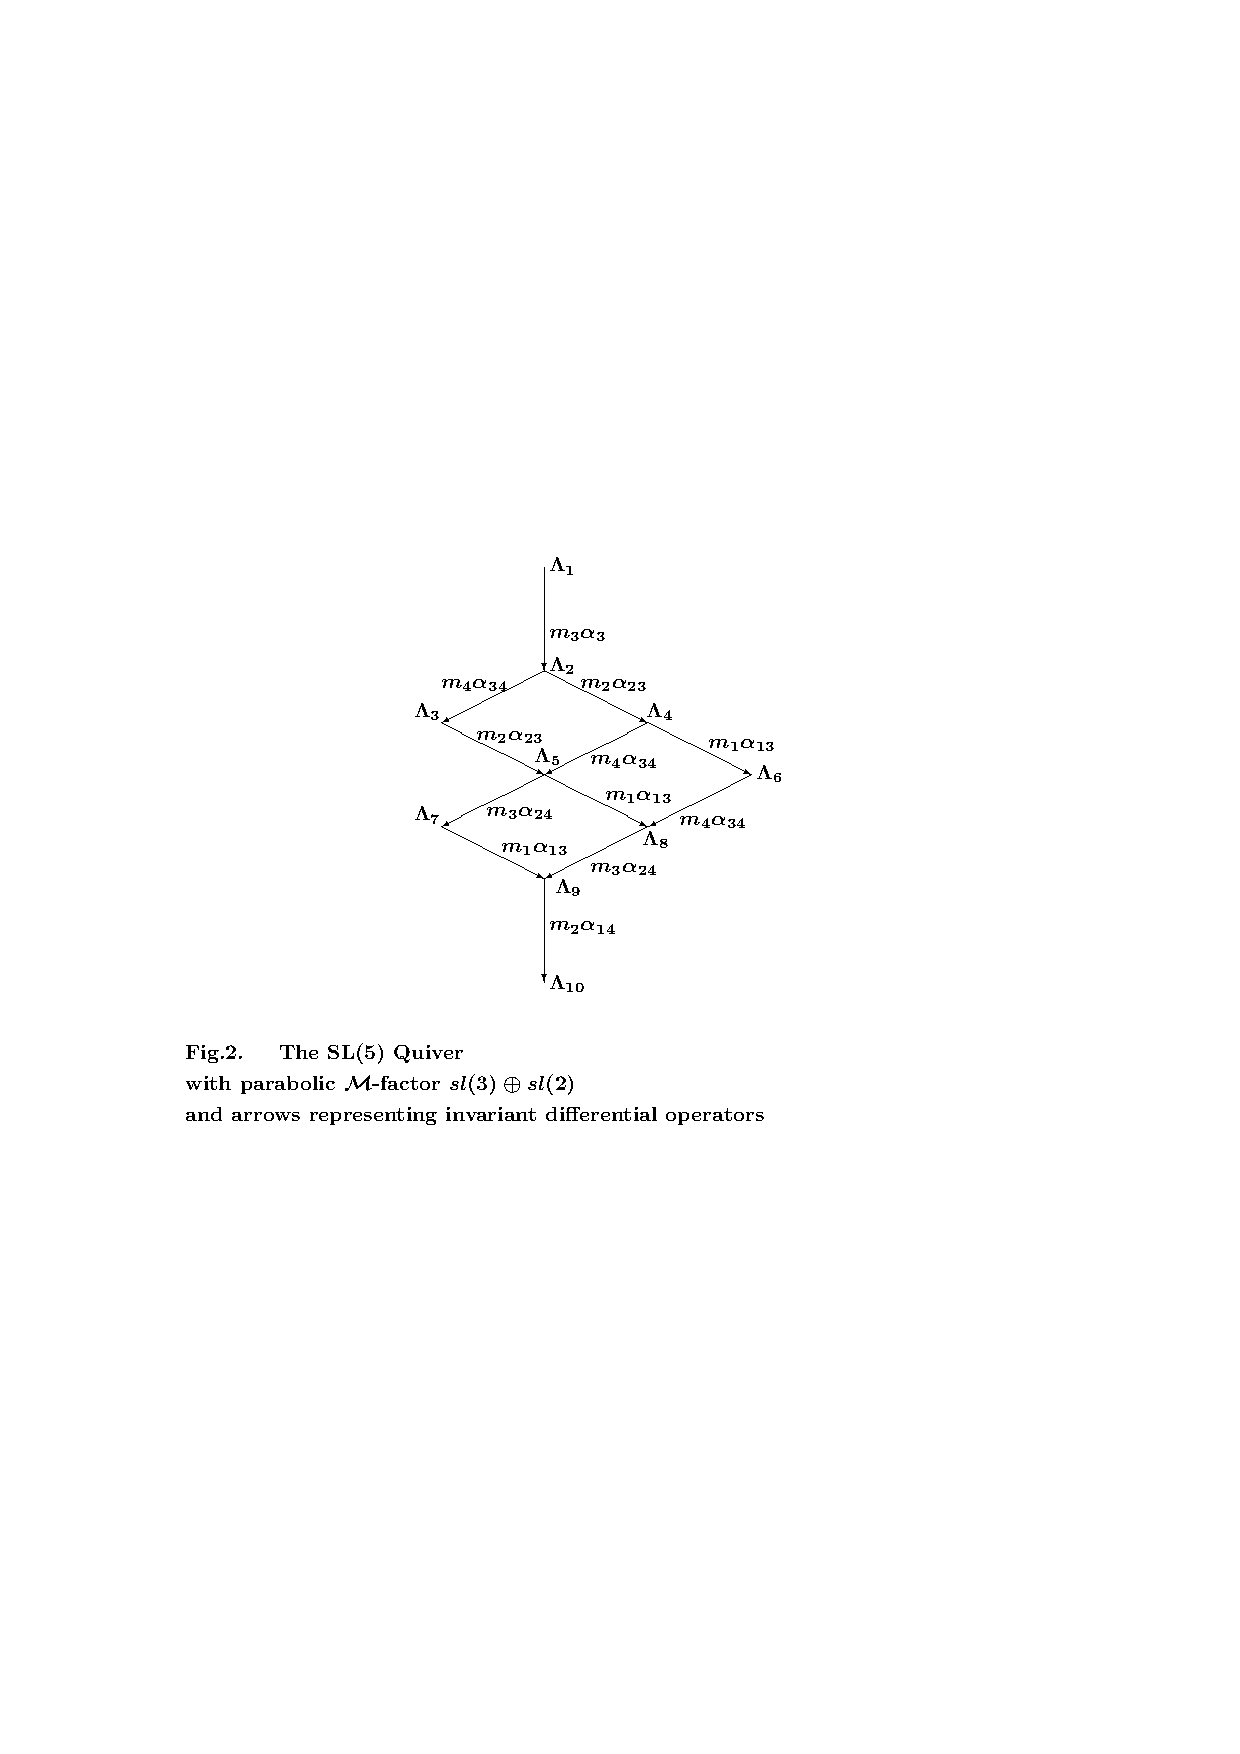
\includegraphics[width=15cm]  {diag-sl5}$$

\newpage

%{\bf  Fig.3.~~~ The SL(7) quiver}

%$$ $$ \vspace{10cm} \includegraphics[bb= 0 -10 500 500, width=14cm]  {diag-sl7}$$  \includegraphics[bb= 0 -10 500 500, width=14cm]  {diag-sl7}$$

$$ .\vspace{-20cm}  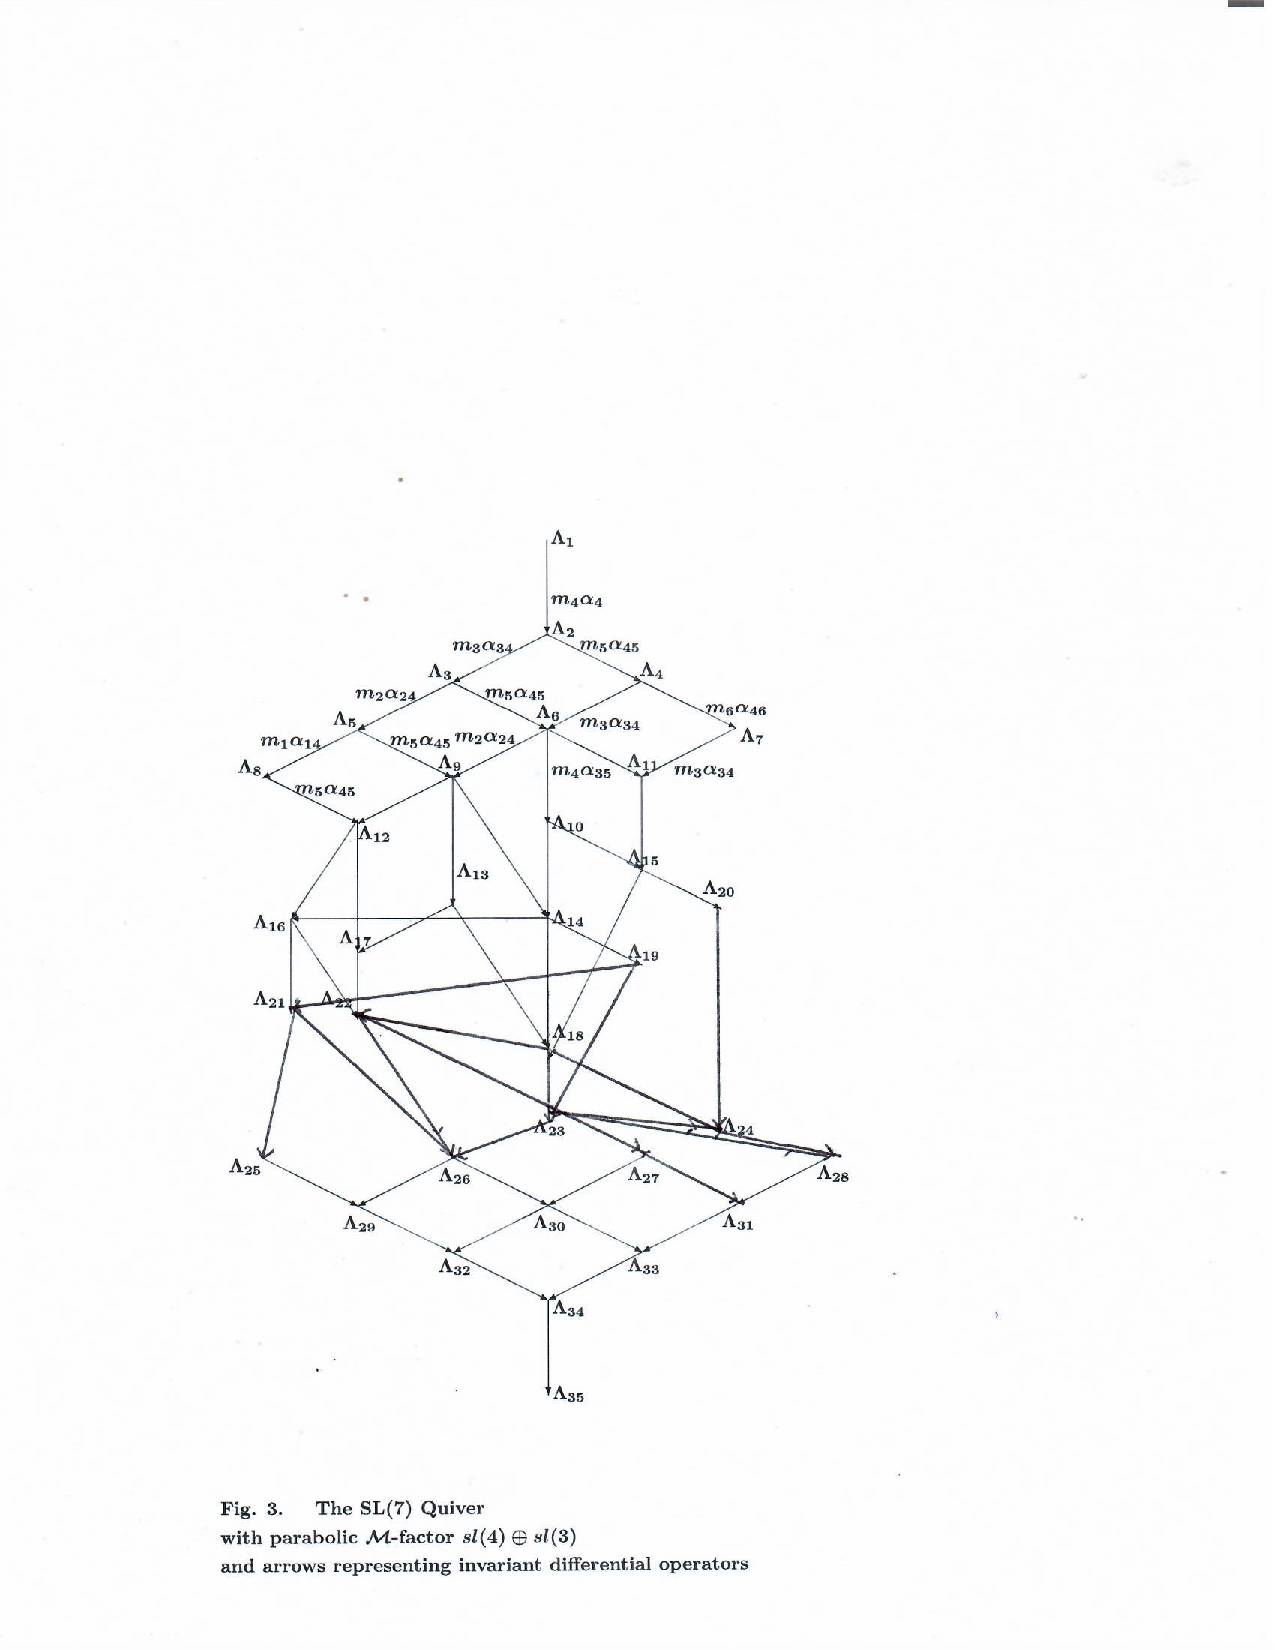
\includegraphics[width=15cm]  {diag-sl77}$$

\end{document}



